\documentclass[a4paper,twoside,11pt]{article}
\usepackage{pstricks}
\usepackage{fancybox}
\usepackage{amsfonts}
\usepackage{ifpdf}
% \usepackage{minitoc}
% \setcounter{minitocdepth}{2}
\usepackage[bookmarks=true,
            bookmarksnumbered=true,
            bookmarksopen=false,
            plainpages=false,
            pdfpagelabels,
            colorlinks,
            citecolor=red,
            linkcolor=blue]{hyperref}
\usepackage{html}
\usepackage{ifthen}
\usepackage{graphicx}
\newtheorem{theorem}{Theorem}
\newtheorem{corollary}{Corollary}
\usepackage{rotating}
\usepackage{microtype}
\usepackage{minted}
\usemintedstyle{friendly}
\definecolor{bg}{rgb}{0.95,0.95,0.95}
\usepackage{breakurl}
\usepackage{mathpazo}
\usepackage[english]{babel}
\ifpdf
\newmintinline[fortinline]{fortran}{}
\else%
\def\fortinline{\lstinline[basicstyle=\ttfamily,language=fortran]}
\fi

%\newboolean{mtc}
%\setboolean{mtc}{true}

\pdfoutput=1
\relax
\pdfcompresslevel=0             %-- 0 = none, 9 = best
\pdfinfo{                       %-- Info dictionary of PDF output  /Author (PD, DdS, SF)
  /Title    (Algebraic MultiGrid Preconditioners Package
             based on PSBLAS, V. 1.0)
  /Subject  (MultiGrid Parallel Preconditioners Package)
  /Keywords (Parallel Numerical Software, Algebraic MultiGrid Preconditioners, Sparse Iterative Solvers, PSBLAS, MPI)
  /Creator  (pdfLaTeX)
  /Producer ($Id: userguide.tex 2021-03-01 Pasqua D'Ambra, Fabio Durastante,
             Salvatore Filippone$)
}
\pdfcatalog{ %-- Catalog dictionary of PDF output.
%  /URI (http://ce.uniroma2.it/psblas)
}

\setlength\textwidth{1.15\textwidth}
\setlength\oddsidemargin{0.3in}
\setlength\evensidemargin{0.2in}
% \newlength{\centeroffset}
% \setlength{\centeroffset}{0.5\oddsidemargin}
% \addtolength{\centeroffset}{0.5\evensidemargin}
% \addtolength{\textwidth}{-\centeroffset}
\pagestyle{myheadings}

\newcounter{subroutine}[subsection]
\newcounter{example}[subroutine]
\makeatletter
\def\subroutine{\@ifstar{\@subroutine}{\clearpage\@subroutine}}%
\def\@subroutine#1#2{%
\stepcounter{subroutine}%
      \section*{\flushleft #1---#2 \endflushleft}%
      \addcontentsline{toc}{subsection}{#1}%
      \markright{#1}}%
\newcommand{\subsubroutine}[2]{%
\stepcounter{subroutine}%
      \subsection*{\flushleft #1---#2 \endflushleft}%
      \addcontentsline{toc}{subsubsection}{#1}%
      \markright{#1}}%
\newcommand{\examplename}{Example}
\newcommand{\syntaxname}{Syntax}
\def\syntax{\@ifstar{\@ssyntax}{\@syntax}}%
\def\@syntax{\nobreak\section*{\syntaxname}%
     \@ssyntax}%
\def\@ssyntax#1#2{%
  \nobreak
   \setbox\@tempboxa\hbox{#1\ {\em $($#2$)$}}%
   \ifdim \wd\@tempboxa >\hsize
        \setbox\@tempboxa\hbox{\em $($#2$)$}
	\ifdim\wd\@tempboxa >\hsize
          \begin{flushright}#1\ \em$($#2$)$\end{flushright}%
	\else
         \hbox to\hsize{#1\hfil}%
         \hbox to\hsize{\hfil\box\@tempboxa}%
        \fi
     \else
       \hbox to\hsize{\hfil\box\@tempboxa\hfil}%
   \fi\par\vskip\baselineskip}
\makeatother
\newcommand{\example}{\stepcounter{example}%
\section*{\examplename~\theexample}}
\def\bsideways{\sidewaystable}
\def\esideways{\endsidewaystable}

\newcommand{\precdata}{\hyperlink{precdata}{{\tt mld\_prec\_type}}}
\newcommand{\descdata}{\hyperlink{descdata}{{\tt psb\_desc\_type}}}
\newcommand{\spdata}{\hyperlink{spdata}{{\tt psb\_spmat\_type}}}
%\newcommand{\Ref}[1]{\mbox{(\ref{#1})}}

\begin{document}
{
\pdfbookmark{AMG4PSBLAS User's and Reference Guide}{title}
\newlength{\centeroffset}
%\setlength{\centeroffset}{-0.5\oddsidemargin}
%\addtolength{\centeroffset}{0.5\evensidemargin}
%\addtolength{\textwidth}{-\centeroffset}
\thispagestyle{empty}
\vspace*{\stretch{1}}
\noindent\hspace*{\centeroffset}\makebox[0pt][l]{\begin{minipage}{\textwidth}
\flushright
{\Huge\bfseries AMG4PSBLAS\\[.8ex] User's and Reference Guide
}
\noindent\rule[-1ex]{\textwidth}{5pt}\\[2.5ex]
\hfill\emph{\Large A guide for the Algebraic MultiGrid \\[.6ex]
Preconditioners Package based on PSBLAS}
\end{minipage}}

\vspace{\stretch{1}}
\flushleft
\begin{figure*}[htb]
\begin{center}
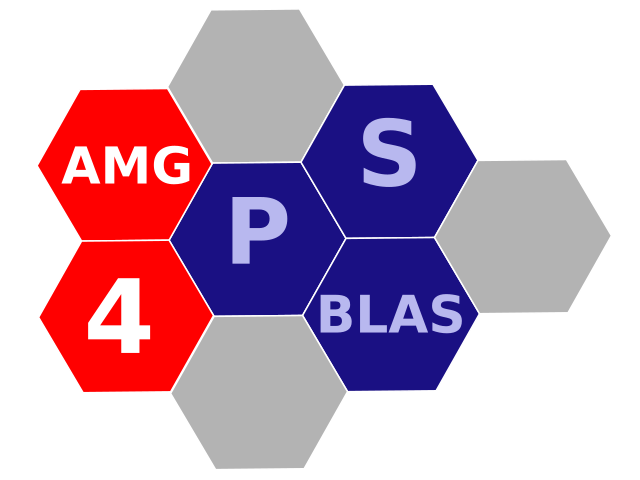
\includegraphics[width=0.6\textwidth]{amg4psblaslibrary.png}
\end{center}
\end{figure*}

\vspace{\stretch{1}}
\noindent\hspace*{\centeroffset}\makebox[0pt][l]{\begin{minipage}{\textwidth}
\flushright
{\large\bfseries Pasqua D'Ambra}\\
\large IAC-CNR, Italy\\[3ex]
{\large\bfseries Fabio Durastante}\\
\large University of Pisa and IAC-CNR\\[3ex]
{\large\bfseries Salvatore Filippone} \\
\large University of Rome Tor-Vergata and IAC-CNR
%\\[10ex]
%\today
\end{minipage}}

\vspace{\stretch{1}}
\noindent\hspace*{\centeroffset}\makebox[0pt][l]{\begin{minipage}{\textwidth}
\flushright
\large Software version: 1.0\\
%\today
\large March 31, 2021
\end{minipage}}
%\addtolength{\textwidth}{\centeroffset}
\vspace{\stretch{2}}
\clearpage
\thispagestyle{empty}
\vspace*{1cm}
\centerline{\emph{\large This page intentionally left blank}}
\clearpage
}
\pagenumbering{roman}   % Roman numbering
\setcounter{page}{1}    % Abstract starts on page i

\section*{Abstract}
\addcontentsline{toc}{section}{Abstract}

\textsc{AMG4PSBLAS (Algebraic MultiGrid Preconditioners Package
based on PSBLAS}) is a package of parallel algebraic multilevel preconditioners included in the PSCToolkit (Parallel Sparse Computation Toolkit) software framework.
It is a progress of a software development project started in 2007, named MLD2P4, which implemented a multilevel version of some domain decomposition preconditioners of additive-Schwarz type and was based on a parallel decoupled version of the well known smoothed
aggregation method to generate the multilevel hierarchy of coarser matrices. In the last years, within the context of the EU-H2020 EoCoE project (Energy Oriented Center of Excellence), the package was extended including new algorithms and functionalities for setup and application of new AMG preconditioners with the final aims of improving efficiency and scalability when tens of thousands cores are
used and of boosting reliability in dealing with general symmetric positive definite linear systems. Due to the significant number of changes and the increase in scope, we decided to rename the package as AMG4PSBLAS.

AMG4PSBLAS has been designed to provide scalable and easy-to-use preconditioners
in the context of the PSBLAS (Parallel Sparse Basic Linear Algebra Subprograms)
computational framework and can be used in conjuction with the Krylov solvers
available in this framework.
Our package is based on a completely algebraic approach and users level interfaces
assume that the system matrix and preconditioners are represented as PSBLAS
distributed sparse matrices.
AMG4PSBLAS enables the user to easily specify different
features of an algebraic multilevel preconditioner, thus allowing to experiment
with different preconditioners for the problem and parallel computers at hand.

The package employs object-oriented design techniques in
Fortran~2003, with interfaces to additional third party libraries
such as MUMPS, UMFPACK, SuperLU, and SuperLU\_Dist, which
can be exploited in building multilevel preconditioners. The parallel
implementation is based on a Single Program Multiple Data (SPMD)
paradigm; the inter-process communication is based on MPI and
is managed mainly through PSBLAS.

This guide provides a brief description of the functionalities and
the user interface of AMG4PSBLAS. 
{
%\cleardoublepage
\clearpage
\thispagestyle{empty}
\vspace*{1cm}
\centerline{\emph{\large This page intentionally left blank}}
\clearpage

\begingroup
\renewcommand*{\thepage}{toc}
\tableofcontents
\endgroup
%\cleardoublepage
\clearpage
\thispagestyle{empty}
\vspace*{1cm}
\centerline{\emph{\large This page intentionally left blank}}
\clearpage
}
\pagenumbering{arabic}  % Arabic numbering
\setcounter{page}{1}    % Chapters start on page 1

\section{General Overview\label{sec:overview}}
\markboth{\textsc{AMG4PSBLAS User's and Reference Guide}}
         {\textsc{\ref{sec:overview} General Overview}}

The \textsc{Algebraic MultiGrid Preconditioners Package based on
PSBLAS} (\textsc{AMG\-4\-PSBLAS}) provides parallel Algebraic MultiGrid (AMG) preconditioners (see, e.g., \cite{Briggs2000,Stuben_01}),
to be used in the iterative solution of  linear systems,
\begin{equation}
Ax=b,
\label{system1}
\end{equation}
where $A$ is a square, real or complex, sparse symmetric positive definite (s.p.d) matrix.
%
%\textbf{NOTA: Caso non simmetrico, aggregazione con $(A+A^T)$ fatta!
%Dovremmo implementare uno smoothed prolongator
%adeguato e fare qualcosa di consistente anche con 1-lev Schwarz.}
%

The preconditioners implemented in AMG4PSBLAS are obtained by combining
3 different types of AMG cycles with smoothers and coarsest-level
solvers. Available multigrid cycles include the V-, W-, and a version of a Krylov-type cycle
(K-cycle)~\cite{Briggs2000,Notay2008}; they can  be
combined with Jacobi hybrid 
%\footnote{see Note 2 in Table~\ref{tab:p_coarse}, p.~28.}
forward/backward Gauss-Seidel, block-Jacobi, and additive Schwarz
smoothers. The  Jacobi, block-Jacobi and
Gauss-Seidel smoothers are also available in the $\ell_1$  version.

An algebraic approach is used to generate a hierarchy of
coarse-level matrices and operators, without explicitly using any information on the
geometry of the original problem, e.g., the discretization of a PDE. To this end,
two different coarsening strategies, based on aggregation, are available:
\begin{itemize}
\item a decoupled version of the  smoothed aggregation procedure
  proposed in~\cite{BREZINA_VANEK,VANEK_MANDEL_BREZINA}, and already
  included in the previous versions of the
  package~\cite{BDDF2007,MLD2P4_TOMS}; 
\item a coupled,  parallel implementation of the  Coarsening based on
  Compatible Weighted Matching introduced   in~\cite{DV2013,DFV2018}
  and described in detail in~\cite{DDF2020};  
\end{itemize}
Either exact or approximate solvers can be used on the coarsest-level
system. We provide interfaces to various  sparse LU factorizations from external 
packages, native incomplete LU and approximate inverse factorizations,
weighted Jacobi, hybrid Gauss-Seidel, block-Jacobi solvers and
a recursive call to preconditioned Krylov methods;  all 
smoothers can be also exploited as one-level preconditioners.

AMG4PSBLAS is written in Fortran~2003, following an
object-oriented design through the exploitation of features
such as abstract data type creation, type extension, functional overloading, and
dynamic memory management.
The parallel implementation is based on a Single Program Multiple Data
(SPMD) paradigm.  Single and
double precision implementations of AMG4PSBLAS are available for both the
real and the complex case, which can be used through a single
interface.

AMG4PSBLAS has been designed to implement scalable and easy-to-use
multilevel preconditioners in the context of the PSBLAS (Parallel Sparse BLAS)
computational framework~\cite{psblas_00,PSBLAS3}. PSBLAS provides basic linear algebra
operators and data management facilities for distributed sparse matrices,
kernels for sequential incomplete factorizations needed for the
parallel block-Jacobi and additive Schwarz smoothers, and 
parallel Krylov solvers which can be used with the AMG4PSBLAS preconditioners.
The choice of PSBLAS has been mainly motivated by the need of having
a portable and efficient software infrastructure implementing ``de facto'' standard
parallel sparse linear algebra kernels, to pursue goals such as performance,
portability, modularity ed extensibility in the development of the preconditioner
package. On the other hand, the implementation of AMG4PSBLAS, which
was driven by the need to face the exascale challenge, has led to some
important  revisions and extentions of the PSBLAS infrastructure. 
The inter-process comunication required by AMG4PSBLAS is encapsulated
in the PSBLAS routines;
therefore, AMG4PSBLAS can be run on any parallel machine where PSBLAS 
implementations are available. In the most recent version of PSBLAS
(release 3.7), a plug-in for GPU is included; it includes CUDA
versions of main vector operations and of sparse matrix-vector
multiplication, so that Krylov methods coupled with AMG4PBLAS
preconditioners    relying on Jacobi and block-Jacobi smoothers with
sparse approximate inverses on the blocks can be efficiently executed
on cluster of GPUs. 

AMG4PSBLAS has a layered and modular software architecture where three main layers can be
identified.  The lower layer consists of the PSBLAS kernels, the middle one implements
the construction and application phases of the preconditioners, and the upper one
provides a uniform interface to all the preconditioners.
This architecture allows for different levels of use of the package:
few black-box routines at the upper layer allow all users to easily
build and apply any preconditioner available in AMG4PSBLAS;
facilities are also available allowing expert users to extend the set of smoothers
and solvers for building new versions of the preconditioners (see
Section~\ref{sec:adding}).

This guide is organized as follows. General information on the distribution of the source
code is reported in Section~\ref{sec:distribution}, while details on the configuration
and installation of the package are given in Section~\ref{sec:building}. The basics for building and applying the
preconditioners with the Krylov solvers implemented in PSBLAS are reported
in~Section~\ref{sec:started}, where the Fortran codes of a few sample programs
are also shown. A reference guide for the user interface routines is provided
in Section~\ref{sec:userinterface}. Information on the extension of the package
through the addition of new smoothers and solvers is reported in Section~\ref{sec:adding}.
The error handling mechanism used by the package
is briefly described in Section~\ref{sec:errors}. The copyright terms concerning the
distribution and modification of AMG4PSBLAS are reported in Appendix~\ref{sec:license}.

%%% Local Variables:
%%% mode: latex
%%% TeX-master: "userguide"
%%% End:

\section{Code Distribution\label{sec:distribution}}
\markboth{\textsc{AMG4PSBLAS User's and Reference Guide}}
         {\textsc{\ref{sec:distribution} Code Distribution}}

\noindent
AMG4PSBLAS is available from the web site
\begin{quotation}
\href{https://psctoolkit.github.io/products/amg4psblas/}{https://psctoolkit.github.io/products/amg4psblas/}
\end{quotation}
where contact points for further information can be also found.

The software is available under a modified BSD license, as specified
in Appendix~\ref{sec:license}; please note that some of the optional
third party libraries may be licensed under a different and more
stringent license, most notably the GPL, and this should be taken into
account when treating derived works.

The library defines a version string with the
constant
\[ \verb|amg_version_string_|\]
whose current value is \verb|1.0|.

\subsection*{Contributors}
\begin{itemize}
\item Pasqua D'Ambra, IAC-CNR, IT;			
\item Fabio Durastante, University of Pisa and IAC-CNR, IT;
\item Salvatore  Filippone, University of Rome Tor-Vergata and IAC-CNR, IT;				
\end{itemize}

\subsection*{Citing AMG4PSBLAS}
When use the library, please cite the following:

\ifpdf
\begin{minted}[breakanywhere,fontsize=\small]{bibtex}
@article{DDF2021,
  author = {D'Ambra, Pasqua and Durastante, Fabio and Filippone, Salvatore},
  title = {{{AMG Preconditioners for Linear Solvers towards Extreme Scale}},
  journal = {arXiv e-preprints},
  eprint = {2006.16147v3},
  archivePrefix = {arXiv},
  year={2021}
}

@Misc{psctoolkit-web-page,
  author = {D'Ambra, Pasqua and Durastante, Fabio and Filippone, Salvatore},
  title =  {{PSCToolkit} {W}eb page},
  url =    {https://psctoolkit.github.io/},
  howpublished = {\url{https://psctoolkit.github.io/}},
  year = {2021}
}
\end{minted}
\else
\begin{verbatim}
@article{DDF2021,
       author = {D'Ambra, Pasqua and Durastante, Fabio and Filippone, Salvatore},
       title = {{{AMG Preconditioners for Linear Solvers towards Extreme Scale}},
       journal = {arXiv e-preprints},
       eprint = {2006.16147v3},
       archivePrefix = {arXiv},
       year={2021}
     }

@Misc{psctoolkit-web-page,
       author = {D'Ambra, Pasqua and Durastante, Fabio and Filippone, Salvatore},
       title =  {{PSCToolkit} {W}eb page},
       url =    {https://psctoolkit.github.io/},
       howpublished = {\url{https://psctoolkit.github.io/}},
       year = {2021}
     }
\end{verbatim}
\fi
\section{Configuring and Building AMG4PSBLAS\label{sec:building}}
\markboth{\textsc{AMG4PSBLAS User's and Reference Guide}}
         {\textsc{\ref{sec:building} Configuring and Building AMG4PSBLAS}}
In order to build AMG4PSBLAS it is necessary to set up a Makefile with appropriate
system-dependent variables; this is done by means of the \verb|configure|
script. The distribution also includes the autoconf and automake
sources employed to generate the script, but usually this is not needed
to build the software.

AMG4PSBLAS is implemented almost entirely in Fortran~2003, with some
interfaces to external libraries in C; the Fortran compiler
must support the Fortran~2003 standard plus the extension \verb|MOLD=|
feature, which enhances the usability of \verb|ALLOCATE|.
Most Fortran compilers provide  this feature; in particular, this is
supported by the GNU Fortran compiler, for which we
recommend to use at least version 4.8.
The software defines data types and interfaces for
real and complex data, in both single and double precision.

Building AMG4PSBLAS requires some base libraries (see
Section~\ref{sec:prerequisites}); interfaces to optional third-party
libraries, which extend the functionalities of AMG4PSBLAS (see
Section~\ref{sec:third-party}), are also available.  A number of Linux
distributions (e.g., Ubuntu, Fedora, CentOS) provide precompiled
packages for the prerequisite and optional software. In many cases
these packages are split between a runtime part and a ``developer''
part; in order to build AMG4PSBLAS you need both. A description of the
base and optional software used by AMG4PSBLAS is given in the next sections.

\subsection{Prerequisites\label{sec:prerequisites}}

The following base libraries are needed:
\begin{description}
\item[BLAS] \cite{blas3,blas2,blas1} Many vendors provide optimized versions
  of BLAS; if no vendor version is
  available for a given platform, the ATLAS software
  (\href{http://math-atlas.sourceforge.net}{math-atlas.sourceforge .net})
  may be employed.  The reference BLAS from Netlib
  (\href{http://www.netlib.org/blas}{www.netlib.org/blas}) are meant to define the standard
  behaviour of the BLAS interface, so they are not optimized for any
  particular platform, and should only be used as a last
  resort. Note that BLAS computations form a relatively small part of
  the AMG4PSBLAS/\-PSBLAS; however they are critical when using
  preconditioners based on the MUMPS, UMFPACK or SuperLU third party
  libraries. UMFPACK requires a full LAPACK library; our
experience is that configuring ATLAS for building full LAPACK does not always
work in the expected way. Our advice is first to download the LAPACK tarfile from
\href{http://www.netlib.org/lapack}{www.netlib.org/lapack} and install it independently of ATLAS. In this case,
you need to modify the OPTS and NOOPT definitions for including -fPIC compilation option
in the make.inc file of the LAPACK library.
 \item[MPI] \cite{MPI2,MPI1} A version of MPI is available on most
  high-performance computing systems.
 \item[PSBLAS] \cite{PSBLASGUIDE,psblas_00} Parallel Sparse BLAS (PSBLAS) is
  available from
  \href{https://psctoolkit.github.io/products/psblas/}{psctoolkit.github.io/
    products/psblas/}; version   3.7.0  (or later) is
  required. Indeed, all the prerequisites   listed so far are also
  prerequisites of PSBLAS. 
\end{description}
Please note that the four previous libraries must have Fortran
interfaces compatible with AMG4PSBLAS; usually this means that they
should all be built with the same compiler being used for  AMG4PSBLAS.

If you want to use the PSBLAS support for NVIDIA GPUs, you will also
need:
\begin{description}
 \item[PSBLAS-EXT] Parallel Sparse BLAS (PSBLAS) Extensions, 
  available from
  \href{https://psctoolkit.github.io/products/psblasext/}{psctoolkit.github.io/products/psblasext/}; version   1.3.0  (or later). 
 \item[SPGPU] Sparse CUDA kernels for NVIDIA GPUs; available from
   GitHub, see also
   \href{https://psctoolkit.github.io/products/psblasext/}{psctoolkit.github.io/products/psblasext/}.
 \end{description}
 See also Sec~\ref{sec:gpu-example}.
 
\subsection{Optional third party libraries\label{sec:third-party}}

We provide interfaces to the following third-party software libraries;
note that these are optional, but if you enable them some defaults
for multilevel preconditioners may change to reflect their presence.

\begin{description}
\item[UMFPACK] \cite{UMFPACK}
  A sparse LU factorization package included in the SuiteSparse library, available from
  \url{faculty.cse.tamu.edu/davis/suitesparse.html};
  it provides sequential factorization and triangular system solution for double
  precision real and complex data. We tested version 4.5.4 of SuiteSparse.
  Note that for configuring SuiteSparse you should provide the right path to the BLAS
  and LAPACK libraries in the \verb|SuiteSparse_config/SuiteSparse_config.mk| file.
\item[MUMPS] \cite{MUMPS}
  A sparse LU factorization package available from \url{mumps.enseeiht.fr};
  it provides sequential and parallel factorizations and triangular system solution
  for single and double precision, real and complex data.
  We tested versions 4.10.0 and 5.0.1.
\item[SuperLU] \cite{SUPERLU}
  A sparse LU factorization package available from
  \url{crd.lbl.gov/~xiaoye/SuperLU/}; it provides sequential
  factorization and triangular system solution for single and double precision,
  real and complex data. We tested versions 4.3 and 5.0. If you installed BLAS from
  ATLAS, remember to define the BLASLIB variable in the make.inc file.
 \item[SuperLU\_Dist] \cite{SUPERLUDIST}
   A sparse LU factorization package available
   from the same site as SuperLU; it provides parallel factorization and
   triangular system solution for double precision real and complex data.
   We tested versions 3.3 and 4.2. If you installed BLAS from
   ATLAS, remember to define the BLASLIB variable in the make.inc file and
   to add the \verb|-std=c99| option to the C compiler options.
   Note that this library requires the ParMETIS
   library for parallel graph partitioning and fill-reducing matrix ordering, available from
   \url{glaros.dtc.umn.edu/gkhome/metis/parmetis/overview}.
\end{description}

\subsection{Configuration options}

In order to build AMG4PSBLAS, the first step is to use the \verb|configure| script
in the main directory to generate the necessary makefile.
%\textbf{Sono necessarie le parentesi intorno a s?}

As a minimal example consider the following:
\ifpdf
\begin{minted}[breaklines=true,bgcolor=bg,fontsize=\small]{console}
./configure --with-psblas=PSB-INSTALL-DIR
\end{minted}
\else
\begin{verbatim}
./configure --with-psblas=PSB-INSTALL-DIR
\end{verbatim}
\fi
which assumes that the various MPI compilers and support libraries are
available in the standard directories on the system, and specifies
only the PSBLAS install  directory (note that the latter directory must
be specified with an {\em absolute} path).
The full set of options may be looked at by issuing the command
\verb|./configure --help|, which produces:
\ifpdf
\inputminted[breaklines=true,bgcolor=bg,fontsize=\small]{console}{../configureout.txt}
\else
\lstinputlisting{../configureout.txt}
\fi
For instance, if a user has built and installed PSBLAS 3.7 under the
\verb|/opt| directory and is
using the SuiteSparse package (which includes UMFPACK), then AMG4PSBLAS
might be configured with:
\ifpdf
\begin{minted}[breaklines=true,bgcolor=bg,fontsize=\small]{console}
./configure --with-psblas=/opt/psblas-3.7/ --with-umfpackincdir=/usr/include/suitesparse/
\end{minted}
\else
\begin{verbatim}
./configure --with-psblas=/opt/psblas-3.7/ \
--with-umfpackincdir=/usr/include/suitesparse/
\end{verbatim}
\fi
Once the configure script has completed execution, it will have
generated the file \verb|Make.inc| which will then be used by all
Makefiles in the directory tree; this file will be copied in the
install directory under the name \verb|Make.inc.AMG4PSBLAS|.

To use the MUMPS solver package,
the user has to add the appropriate options to the configure script;
by default we are looking for the libraries
\verb|-ldmumps -lsmumps| \verb| -lzmumps -lcmumps -mumps_common -lpord|.
MUMPS often uses additional packages such as ScaLAPACK, ParMETIS,
SCOTCH, as well as enabling OpenMP; in such cases it is necessary to
add linker options with the \verb|--with-extra-libs| configure option.

To build the library the user will now enter
\ifpdf
\begin{minted}[breaklines=true,bgcolor=bg,fontsize=\small]{console}
make
\end{minted}
\else
\begin{verbatim}
make
\end{verbatim}
\fi
followed (optionally) by
\ifpdf
\begin{minted}[breaklines=true,bgcolor=bg,fontsize=\small]{console}
make install
\end{minted}
\else
\begin{verbatim}
make install
\end{verbatim}
\fi
\subsection{Bug reporting}
If you find any bugs in our codes, please report them through our
issues page on \\[2mm]
\url{https://github.com/psctoolkit/amg4psblas/issues}\\

To enable us to track the bug, please provide a log from the failing
application, the test conditions, and ideally a self-contained test
program reproducing the issue.

\subsection{Example and test programs\label{sec:ex_and_test}}
The package contains the \verb|examples| and \verb|tests| directories;
both of them are further divided into \verb|fileread| and
\verb|pdegen| subdirectories. Their purpose is as follows:
\begin{description}
\item[\tt examples] contains a set of simple example programs with a
  predefined choice of preconditioners, selectable via integer
  values. These are intended to get  acquainted with the
  multilevel preconditioners available in AMG4PSBLAS.
\item[\tt tests] contains a set of more sophisticated examples that
  will allow the user, via the input files in the \verb|runs|
  subdirectories, to experiment with the full range of preconditioners
  implemented in the package.
\end{description}
The \verb|fileread| directories contain sample programs that read
sparse matrices from files, according to the Matrix Market or the
Harwell-Boeing storage format; the \verb|pdegen| programs generate
matrices in full parallel mode from the discretization of a sample partial
differential equation.

\section{Getting Started\label{sec:started}}
\markboth{\textsc{AMG4PSBLAS User's and Reference Guide}}
         {\textsc{\ref{sec:started} Getting Started}}

We describe the basics for building and applying AMG4PSBLAS one-level and multilevel
(i.e., AMG) preconditioners with the Krylov solvers included in PSBLAS \cite{PSBLASGUIDE}.
The following steps are required:
\begin{enumerate}
\item \emph{Declare the preconditioner data structure}. It is a derived data type,
  \verb|amg_|\-\emph{x}\verb|prec_| \verb|type|, where \emph{x} may be \verb|s|, \verb|d|, \verb|c|
	or \verb|z|, according to the basic data type of the sparse matrix
	(\verb|s| = real single precision; \verb|d| = real double precision;
	\verb|c| = complex single precision; \verb|z| = complex double precision).
	This data structure is accessed by the user only through the AMG4PSBLAS routines,
	following an object-oriented approach.
\item \emph{Allocate and initialize the preconditioner data structure, according to
	a preconditioner type chosen by the user}. This is performed by the routine
	\verb|init|, which also sets defaults for each preconditioner
	type selected by the user. The preconditioner types and the defaults associated
	with them are given in Table~\ref{tab:precinit}, where the strings used by
	\verb|init| to identify the preconditioner types are also given.
	Note that these strings are valid also if uppercase letters are substituted by
	corresponding lowercase ones.

\item \emph{Modify the selected preconditioner type, by properly setting
  preconditioner parameters.} This is performed by the routine \verb|set|.
  This routine must be called only if the user wants to modify the default values
  of the parameters associated with the selected preconditioner type, to obtain a variant
  of that preconditioner. Examples of use of \verb|set| are given in
  Section~\ref{sec:examples}; a complete list of all the
  preconditioner parameters and their allowed and default values is provided in
  Section~\ref{sec:userinterface}, Tables~\ref{tab:p_cycle}-\ref{tab:p_smoother_1}.
\item \emph{Build the preconditioner for a given matrix}. If the selected preconditioner
 is multilevel, then two steps must be performed, as specified next.
\begin{enumerate}
\item[4.1] \emph{Build the aggregation hierarchy for a given matrix.} This is
performed by the routine \verb|hierarchy_build|.
\item[4.2] \emph{Build the preconditioner for a given matrix.} This is performed
by the routine \verb|smoothers_build|.
\end{enumerate}
 If the selected preconditioner is one-level, it is built in a single step,
performed by the routine \verb|bld|.
\item \emph{Apply the preconditioner at each iteration of a Krylov solver.}
  This is performed by the method \verb|apply|. When using the PSBLAS Krylov solvers,
  this step is completely transparent to the user, since \verb|apply| is called
  by the PSBLAS routine implementing the Krylov solver (\verb|psb_krylov|).
\item \emph{Free the preconditioner data structure}. This is performed by
  the routine \verb|free|. This step is complementary to step 1 and should
  be performed when the preconditioner is no more used.
\end{enumerate}

All the previous routines are available as methods of the preconditioner object.
A detailed description of them is given in Section~\ref{sec:userinterface}.
Examples showing the basic use of AMG4PSBLAS are reported in Section~\ref{sec:examples}.

\begin{table}[h!]
\begin{center}
%{\small
\begin{tabular}{|l|p{1.8cm}|p{8.2cm}|}
\hline
\textsc{type}       & \textsc{string} & \textsc{default preconditioner} \\ \hline
No preconditioner &\verb|'NONE'|& Considered  to use the PSBLAS
                                    Krylov solvers with no preconditioner. \\ \hline
Diagonal          & \verb|'DIAG'| or \verb|'JACOBI'| & Diagonal preconditioner.
                         For any zero diagonal entry of the matrix to be preconditioned,
                         the corresponding entry of the preconditioner is set to~1.\\ \hline
Gauss-Seidel      & \verb|'GS'|     & Hybrid Gauss-Seidel (forward), that is,
                                      global block Jacobi with
                                      Gauss-Seidel as local solver.\\ \hline
Symmetrized Gauss-Seidel      & \verb|'FBGS'|     & Symmetrized hybrid Gauss-Seidel,that is,
                                      forward Gauss-Seidel followed by
                                                    backward Gauss-Seidel.\\ \hline
Block Jacobi      & \verb|'BJAC'| & Block-Jacobi with ILU(0) on the local blocks.\\ \hline
Additive Schwarz  & \verb|'AS'|   & Additive Schwarz (AS),
                                    with overlap~1 and ILU(0) on the local blocks. \\ \hline
Multilevel        &\verb|'ML'|    & V-cycle with one hybrid forward Gauss-Seidel
                                    (GS) sweep as pre-smoother and one hybrid backward
                                    GS sweep as post-smoother, basic smoothed aggregation
                                   as coarsening algorithm, and LU (plus triangular solve)
                                   as coarsest-level solver. See the default values in
                                   Tables~\ref{tab:p_cycle}-\ref{tab:p_smoother_1}
                                   for further details of the preconditioner. \\
\hline
\end{tabular}
%}
\caption{Preconditioner types, corresponding strings and default choices.
\label{tab:precinit}}
\end{center}
\end{table}

Note that the module \verb|amg_prec_mod|, containing the definition of the
preconditioner data type and the interfaces to the routines of AMG4PSBLAS,
must be used in any program calling such routines.
The modules \verb|psb_base_mod|, for the sparse matrix and communication descriptor
data types, and \verb|psb_krylov_mod|, for interfacing with the
Krylov solvers, must be also used (see Section~\ref{sec:examples}). \\

\textbf{Remark 1.} Coarsest-level solvers based on the LU factorization,
such as those implemented in UMFPACK, MUMPS, SuperLU, and SuperLU\_Dist,
usually lead to smaller numbers of preconditioned Krylov
iterations than inexact solvers, when the linear system comes from
a standard discretization of basic scalar elliptic PDE problems. However,
this does not necessarily correspond to the smallest execution time
on parallel computers.


{\em DA MODIFICARE PER INSERIRE TIPO DI AGGREGAZIONE}

\subsection{Examples\label{sec:examples}}

The code reported in Figure~\ref{fig:ex1} shows how to set and apply the default
multilevel preconditioner available in the real double precision version
of AMG4PSBLAS (see Table~\ref{tab:precinit}). This preconditioner is chosen
by simply specifying \verb|'ML'| as the second argument of \verb|P%init|
(a call to \verb|P%set| is not needed) and is applied with the CG
solver provided by PSBLAS (the matrix of the system to be solved is
assumed to be positive definite). As previously observed, the modules
\verb|psb_base_mod|, \verb|amg_prec_mod| and \verb|psb_krylov_mod|
must be used by the example program.

The part of the code concerning the
reading and assembling of the sparse matrix and the right-hand side vector, performed
through the PSBLAS routines for sparse matrix and vector management, is not reported
here for brevity; the statements concerning the deallocation of the PSBLAS
data structure are neglected too.
The complete code can be found in the example program file \verb|amg_dexample_ml.f90|,
in the directory \verb|examples/fileread| of the AMG4PSBLAS implementation (see
Section~\ref{sec:ex_and_test}). A sample test problem along with the relevant
input data is available in \verb|examples/fileread/runs|.
For details on the use of the PSBLAS routines, see the PSBLAS User's
Guide~\cite{PSBLASGUIDE}.

The setup and application of the default multilevel preconditioner
for the real single precision and the complex, single and double
precision, versions are obtained with straightforward modifications of the previous
example (see Section~\ref{sec:userinterface} for details). If these versions are installed,
the corresponding codes are available in \verb|examples/fileread/|.

\begin{figure}[tbp]
\begin{center}
\begin{minipage}{.90\textwidth}
{\small
\begin{verbatim}
  use psb_base_mod
  use amg_prec_mod
  use psb_krylov_mod
... ...
!
! sparse matrix
  type(psb_dspmat_type) :: A
! sparse matrix descriptor
  type(psb_desc_type)   :: desc_A
! preconditioner
  type(amg_dprec_type)  :: P
! right-hand side and solution vectors
  type(psb_d_vect_type) :: b, x
... ...
!
! initialize the parallel environment
  call psb_init(ictxt)
  call psb_info(ictxt,iam,np)
... ...
!
! read and assemble the spd matrix A and the right-hand side b
! using PSBLAS routines for sparse matrix / vector management
... ...
!
! initialize the default multilevel preconditioner, i.e. V-cycle
! with basic smoothed aggregation, 1 hybrid forward/backward
! GS sweep as pre/post-smoother and UMFPACK as coarsest-level
! solver
  call P%init('ML',info)
!
! build the preconditioner
  call P%hierarchy_build(A,desc_A,info)
  call P%smoothers_build(A,desc_A,info)

!
! set the solver parameters and the initial guess
  ... ...
!
! solve Ax=b with preconditioned CG
  call psb_krylov('CG',A,P,b,x,tol,desc_A,info)
  ... ...
!
! deallocate the preconditioner
  call P%free(info)
!
! deallocate other data structures
  ... ...
!
! exit the parallel environment
  call psb_exit(ictxt)
  stop
\end{verbatim}
}
\end{minipage}
\caption{setup and application of the default multilevel preconditioner (example 1).
\label{fig:ex1}}
\end{center}
\end{figure}

Different versions of the multilevel preconditioner can be obtained by changing
the default values of the preconditioner parameters. The code reported in
Figure~\ref{fig:ex2} shows how to set a V-cycle preconditioner
which applies 1 block-Jacobi sweep as pre- and post-smoother,
and solves the coarsest-level system with 8 block-Jacobi sweeps.
Note that the ILU(0) factorization (plus triangular solve) is used as
local solver for the block-Jacobi sweeps, since this is the default associated
with block-Jacobi and set by~\verb|P%init|.
Furthermore, specifying block-Jacobi as coarsest-level
solver implies that the coarsest-level matrix is distributed
among the processes.
Figure~\ref{fig:ex3} shows how to set a W-cycle preconditioner which
applies 2 hybrid Gauss-Seidel sweeps as pre- and post-smoother,
and solves the coarsest-level system with the multifrontal LU factorization
implemented in MUMPS. It is specified that the coarsest-level
matrix is distributed, since MUMPS can be used on both
replicated and distributed matrices, and by default
it is used on replicated ones.
%Note the use of the parameter \verb|pos|
%to specify a property only for the pre-smoother or the post-smoother
%(see Section~\ref{sec:precset} for more details).
The code fragments shown in Figures~\ref{fig:ex2} and \ref{fig:ex3} are
included in the example program file \verb|amg_dexample_ml.f90| too.

Finally, Figure~\ref{fig:ex4} shows the setup of a one-level
additive Schwarz preconditioner, i.e., RAS with overlap 2.
Note also that a Krylov method different from CG must be used to solve
the preconditioned system, since the preconditione in nonsymmetric.
The corresponding example program is available in the file
\verb|amg_dexample_1lev.f90|.

For all the previous preconditioners, example programs where the sparse matrix and
the right-hand side are generated by discretizing a PDE with Dirichlet
boundary conditions are also available in the directory \verb|examples/pdegen|.

\begin{figure}[tbh]
\begin{center}
\begin{minipage}{.90\textwidth}
{\small
\begin{verbatim}
... ...
! build a V-cycle preconditioner with 1 block-Jacobi sweep (with
! ILU(0) on the blocks) as pre- and post-smoother, and 8  block-Jacobi
! sweeps (with ILU(0) on the blocks) as coarsest-level solver
  call P%init('ML',info)
  call_P%set('SMOOTHER_TYPE','BJAC',info)
  call P%set('COARSE_SOLVE','BJAC',info)
  call P%set('COARSE_SWEEPS',8,info)
  call P%hierarchy_build(A,desc_A,info)
  call P%smoothers_build(A,desc_A,info)
... ...
\end{verbatim}
}
\end{minipage}

\caption{setup of a multilevel preconditioner\label{fig:ex2}}
\end{center}
\end{figure}

\begin{figure}[h!]
\begin{center}
\begin{minipage}{.90\textwidth}
{\small
\begin{verbatim}
... ...
! build a W-cycle preconditioner with 2 hybrid Gauss-Seidel sweeps
! as pre- and post-smoother, a distributed coarsest
! matrix, and MUMPS as coarsest-level solver
  call P%init('ML',info)
  call P%set('ML_CYCLE','WCYCLE',info)
  call P%set('SMOOTHER_TYPE','FBGS',info)
  call P%set('SMOOTHER_SWEEPS',2,info)
  call P%set('COARSE_SOLVE','MUMPS',info)
  call P%set('COARSE_MAT','DIST',info)
  call P%hierarchy_build(A,desc_A,info)
  call P%smoothers_build(A,desc_A,info)
... ...
\end{verbatim}
}
\end{minipage}
\caption{setup of a multilevel preconditioner\label{fig:ex3}}
\end{center}
\end{figure}

\begin{figure}[h!]
\begin{center}
\begin{minipage}{.90\textwidth}
{\small
\begin{verbatim}
... ...
! set RAS with overlap 2 and ILU(0) on the local blocks
  call P%init('AS',info)
  call P%set('SUB_OVR',2,info)
  call P%bld(A,desc_A,info)
... ...
! solve Ax=b with preconditioned BiCGSTAB
  call psb_krylov('BICGSTAB',A,P,b,x,tol,desc_A,info)
\end{verbatim}
}
\end{minipage}
\caption{setup of a one-level Schwarz preconditioner.\label{fig:ex4}}
\end{center}
\end{figure}


%%% Local Variables:
%%% mode: latex
%%% TeX-master: "userguide"
%%% End:

\section{User Interface\label{sec:userinterface}}
\markboth{\textsc{AMG4PSBLAS User's and Reference Guide}}
         {\textsc{\ref{sec:userinterface} User Interface}}

The basic user interface of AMG4PBLAS consists of eight methods. The six
methods \fortinline|init|, \fortinline|set|, \fortinline|build|,
\fortinline|hierarchy_build|, \fortinline|smoothers_build| and \fortinline|apply|
encapsulate all the functionalities for the setup and the application
of any multilevel and one-level preconditioner implemented in the
package.
The method \fortinline|free| deallocates the preconditioner data structure, while
\fortinline|descr| prints a description of the preconditioner setup by the user.
For backward compatibility,  methods are also accessible as
stand-alone subroutines.

For each method, the same user interface is overloaded with
respect to the real/complex  and single/double precision data;
arguments with appropriate data types must be passed to the method, i.e.,
\begin{itemize}
\item the sparse matrix data structure, containing the matrix to be
  preconditioned, must be of type \verb|psb_|\emph{x}\verb|spmat_type| 
  with \emph{x} = \verb|s| for real single precision, \emph{x} =
  \verb|d| for real double precision, \emph{x} = \verb|c| for complex
  single precision, \emph{x} = \verb|z| for complex double precision;
\item the preconditioner data structure must be of type
  \verb|amg_|\emph{x}\verb|prec_type|, with \emph{x} =
  \verb|s|, \verb|d|, \verb|c|, \verb|z|, according to the sparse
  matrix data structure;
\item the arrays containing the vectors $v$ and $w$ involved in
  the preconditioner application $w=B^{-1}v$ must be of type
  \verb|psb_|\emph{x}\verb|vect_type| with \emph{x} =
  \verb|s|, \verb|d|, \verb|c|, \verb|z|, in a manner completely
  analogous to the sparse matrix type;
\item real parameters defining the preconditioner must be declared
  according to the precision of the sparse matrix and preconditioner
  data structures (see Section~\ref{sec:precset}).
\end{itemize}
A description of each method is given in the remainder of this section.

\clearpage

\subsection{Method init\label{sec:precinit}}

\begin{center}
\fortinline|call p%init(contxt,ptype,info)|
\end{center}

\noindent
This method allocates and initializes the preconditioner
\fortinline|p|, according to the preconditioner type chosen by the user.

{\vskip1.5\baselineskip\noindent\large\bfseries Arguments} \smallskip

\begin{tabular}{p{1.2cm}p{12cm}}

  \fortinline|contxt| & \fortinline|type(psb_ctxt_type), intent(in)|.\\
          &  The communication context.\\
\fortinline|ptype|  & \fortinline|character(len=*), intent(in)|.\\
              & The type of preconditioner. Its values are specified
              in Table~\ref{tab:precinit}.\\
              & Note that strings are case insensitive.\\
\fortinline|info|   & \fortinline|integer, intent(out)|.\\
              & Error code. If no error, 0 is returned. See Section~\ref{sec:errors} for details.\\

\end{tabular}




\clearpage

\subsection{Method set\label{sec:precset}}

\begin{center}
\fortinline|call p%set(what,val,info [,ilev, ilmax, pos, idx])|
\end{center}

\noindent
This method sets the parameters defining the preconditioner \fortinline|p|. More
precisely, the parameter identified by \fortinline|what| is assigned the value
contained in \fortinline|val|.

{\vskip1.5\baselineskip\noindent\large\bfseries Arguments} \smallskip

\begin{tabular}{p{1.2cm}p{12cm}}
\fortinline|what|   & \fortinline|character(len=*)|. \\
              & The parameter to be set. It can be specified through its name;
                the string is case-insensitive. See
                Tables~\ref{tab:p_cycle}-\ref{tab:p_smoother_1}.\\
\fortinline|val |   & \fortinline|integer| \emph{or} \fortinline|character(len=*)| \emph{or}
                \fortinline|real(psb_spk_)| \emph{or} \fortinline|real(psb_dpk_)|,
                \fortinline|intent(in)|.\\
              & The value of the parameter to be set. The list of allowed
                values and the corresponding data types is given in
                Tables~\ref{tab:p_cycle}-\ref{tab:p_smoother_1}.
                When the value is of type \fortinline|character(len=*)|,
                it is also treated as case insensitive.\\
\fortinline|info|   & \fortinline|integer, intent(out)|.\\
              & Error code. If no error, 0 is returned. See Section~\ref{sec:errors}
                for details.\\
\fortinline|ilev|   & \fortinline|integer, optional, intent(in)|.\\
              & For the multilevel preconditioner, the level at which the
                preconditioner parameter has to be set.
                The levels are numbered in increasing
                order starting from the finest one, i.e., level 1 is the finest level.
                If \fortinline|ilev| is not present, the parameter identified by \fortinline|what|
                is set at all  levels that are appropriate (see
                Tables~\ref{tab:p_cycle}-\ref{tab:p_smoother_1}).\\
\fortinline|ilmax|   & \fortinline|integer, optional, intent(in)|.\\
              & For the multilevel preconditioner, when both
                \fortinline|ilev| and \fortinline|ilmax| are present, the settings
                are applied at all levels \fortinline|ilev:ilmax|. When
                \fortinline|ilev| is present but \fortinline|ilmax| is not, then
                the default is \fortinline|ilmax=ilev|.
                The levels are numbered in increasing
                order starting from the finest one, i.e., level 1 is the finest level. \\
\fortinline|pos|   & \fortinline|character(len=*), optional, intent(in)|.\\
              & Whether the other arguments apply only to the pre-smoother (\fortinline|'PRE'|)
                or to the post-smoother (\fortinline|'POST'|). If \fortinline|pos| is not present,
                the other arguments are applied to both smoothers.
                If the preconditioner is one-level or the parameter identified by \fortinline|what|
                does not concern the smoothers, \fortinline|pos| is ignored.\\
\fortinline|idx|   & \fortinline|integer, optional, intent(in)|.\\
              & An auxiliary input argument that can be passed to the
                underlying objects.
\end{tabular}


\noindent
%However, in this case the optional arguments \fortinline|ilev|,
%\fortinline|ilmax|, \fortinline|pos| and \fortinline|idx|
%cannot be used. \\

A variety of preconditioners can be obtained by setting the
appropriate preconditioner parameters. These parameters  can be
logically divided into four groups, i.e., parameters defining 
\begin{enumerate}
	\item the type of multilevel cycle and how many cycles must be applied;
        \item the coarsening algorithm;
        \item the coarse-space correction at the coarsest level (for multilevel
                 preconditioners only);
	\item the smoother of the multilevel preconditioners, or the one-level
                  preconditioner.	
\end{enumerate}
A list of the parameters that can be set, along with their allowed and
default values, is given in Tables~\ref{tab:p_cycle}-\ref{tab:p_smoother_1}.\\

\textbf{Remark 2.} A smoother is usually obtained by combining two objects:
a smoother (\fortinline|'SMOOTHER_TYPE'|) and a local solver (\fortinline|'SUB_SOLVE'|),
as specified in Tables~\ref{tab:p_smoother}-\ref{tab:p_smoother_1}.
For example, the block-Jacobi smoother using
ILU(0) on the blocks is obtained by combining the block-Jacobi smoother
object with the ILU(0) solver object. Similarly,
the hybrid Gauss-Seidel smoother (see Note in Table~\ref{tab:p_smoother})
is obtained by combining the block-Jacobi smoother object with a single sweep
of the Gauss-Seidel solver object, while the point-Jacobi smoother is the
result of combining the block-Jacobi smoother object with a single sweep
of the point-Jacobi solver object. However, for simplicity, shortcuts are
provided to set point-Jacobi, hybrid (forward) Gauss-Seidel, and
hybrid backward Gauss-Seidel, i.e., the previous smoothers can be defined
just by setting \fortinline|'SMOOTHER_TYPE'| to certain specific
values (see Tables~\ref{tab:p_smoother}), without the need to set
\fortinline|'SUB_SOLVE'| as well.

The smoother and solver objects are arranged in a
hierarchical manner. When specifying a smoother object, its parameters,
including the local solver, are set to their default values, and when a solver
object is specified, its defaults are also set, overriding in both
cases any previous settings even if explicitly specified. Therefore if
the user sets a smoother, and wishes to use a solver
different from  the default one, the call to set the solver must come
\emph{after} the call to set the smoother.

Similar considerations apply to the point-Jacobi, Gauss-Seidel and block-Jacobi
coarsest-level solvers, and shortcuts are available
in this case too (see Table~\ref{tab:p_coarse}). \\

\textbf{Remark 3.} Many of the coarsest-level solvers cannot be used
with both the replicated and distributed coarsest-matrix layout; 
therefore, setting the solver after the layout may change the layout.
Similarly, setting the layout after the solver may change the solver.

More precisely, UMFPACK and SuperLU require the coarsest-level
matrix to be replicated, while SuperLU\_Dist requires it to be distributed.
In these cases, setting the coarsest-level solver implies that
the layout is redefined according to the solver, ovverriding any
previous settings. MUMPS,  point-Jacobi,
hybrid Gauss-Seidel and block-Jacobi can be applied to
replicated and distributed matrices, thus their choice
does not modify any previously specified layout.
It is worth noting that, when the matrix is replicated,
the point-Jacobi, hybrid Gauss-Seidel and block-Jacobi solvers
reduce to the corresponding local solver objects (see Remark~2).
For the point-Jacobi and Gauss-Seidel solvers, these objects
correspond to a \emph{single} point-Jacobi sweep and a \emph{single}
Gauss-Seidel sweep, respectively, which are very poor solvers.

On the other hand, the distributed layout can be used with any solver
but UMFPACK and SuperLU; therefore, if any of these two solvers has already
been selected, the coarsest-level solver is changed to block-Jacobi,
with the previously chosen solver applied to the local blocks.
Likewise, the replicated layout can be used with any solver but SuperLu\_Dist;
therefore, if SuperLu\_Dist has been previously set, the coarsest-level
solver is changed to the default sequential solver.

\textbf{Remark 4.}  The argument \fortinline|idx| can be used to allow finer
control for those solvers; for instance, by specifying the keyword
\fortinline|'MUMPS_IPAR_ENTRY'| and an appropriate value for \fortinline|idx|, it is
possible to set any entry in the MUMPS integer control array.
See also Sec.~\ref{sec:adding}.
%The \verb|what,val| pairs described here are those of the predefined
%moother/solver objects; newly developed solvers may define new pairs
%according to their needs.


\bsideways
\begin{center}
%\begin{tabular}{|p{5cm}|l|p{2.4cm}|p{2.5cm}|p{5cm}|}
\begin{tabular}{|p{3.6cm}|l|p{2.4cm}|p{2.4cm}|p{7.2cm}|}
\hline
\fortinline|what|              & \textsc{data type}        &  \fortinline|val|      &  \textsc{default}  &
\textsc{comments} \\ \hline
\fortinline|'ML_CYCLE'|     & \fortinline|character(len=*)|
                         & \fortinline|'VCYCLE'| \par \fortinline|'WCYCLE'|   \par \fortinline|'KCYCLE'| \par \fortinline|'ADD'|
                         & \fortinline|'VCYCLE'|
                         &Multilevel cycle: V-cycle, W-cycle, K-cycle, and additive composition. \\ \hline
 \fortinline|'OUTER_SWEEPS'| & \fortinline|integer| &
                           Any integer \par number $\ge 1$  & 1 &
                           Number of multilevel cycles. \\ \hline

\end{tabular}
\end{center}
\caption{Parameters defining the multilevel cycle and the number of cycles to
be applied.
\label{tab:p_cycle}}
\esideways

\bsideways
\begin{center}
%\begin{tabular}{|p{5cm}|l|p{2.4cm}|p{2.5cm}|p{5cm}|}
\begin{tabular}{|p{5.7cm}|l|p{2.3cm}|p{2.5cm}|p{6.9cm}|}
\hline
\fortinline|what|              & \textsc{data type}        &  \fortinline|val|      &  \textsc{default}  &
\textsc{comments} \\ \hline
\fortinline|'MIN_COARSE_SIZE_PER_PROCESS'| & \fortinline|integer|
                         & Any number \par $> 0$
                         & $200$
                         & Coarse size threshold per process. The aggregation stops
                            if  the global number of variables of the
                            computed coarsest matrix
                            is lower than or equal to this threshold
                           multiplied by the number of processes (see Note).
                           \\ \hline
\fortinline|'MIN_COARSE_SIZE'| & \fortinline|integer|
                         & Any number \par $> 0$
                         & -1
                         & Coarse size threshold. The aggregation stops
                            if  the global number of variables of the
                            computed coarsest matrix
                            is lower than or equal to this threshold
                           (see Note). If negative, it is ignored in
                           favour of the default for
                           \fortinline|'MIN_COARSE_SIZE_PER_PROCESS'|. 
                           \\ \hline

\fortinline|'MIN_CR_RATIO'| & \fortinline|real|
                         & Any number \par $> 1$
                         & 1.5
                         & Minimum coarsening ratio. The aggregation stops
                            if the ratio between the global matrix dimensions
                            at two consecutive levels is lower than or equal to this
                            threshold (see Note).\\ \hline

\fortinline|'MAX_LEVS'| & \fortinline|integer|
                         & Any integer \par number $> 1$
                         & 20
                         & Maximum number of levels. The aggregation stops
                           if the number of levels reaches this value (see Note). \\ \hline
\fortinline|'PAR_AGGR_ALG'|  & \fortinline|character(len=*)| \hspace*{-3mm}
& \texttt{'DEC'}, \texttt{'SYMDEC'}, \texttt{'COUPLED'}
& \texttt{'DEC'}
& Parallel aggregation algorithm. \par the
\fortinline|SYMDEC| option applies decoupled
aggregation to  the sparsity pattern
of $A+A^T$.\\ \hline
\ifpdf
\phantomcaption
\end{tabular}
\end{center}
\esideways
\bsideways
\ContinuedFloat
\begin{center}
\begin{tabular}{|p{5.7cm}|l|p{2.3cm}|p{2.5cm}|p{5.9cm}|}
\hline
\fortinline|what|              & \textsc{data type}        &  \fortinline|val|      &  \textsc{default}  &
\textsc{comments} \\ \hline
\fi
\fortinline|'AGGR_TYPE'|  & \fortinline|character(len=*)| \hspace*{-3mm}
& \fortinline|'SOC1'| &
\fortinline|'SOC1'|,
\fortinline|'SOC2'|,
\fortinline|'MATCHBOXP'|
& Type of aggregation algorithm: currently,
for the decoupled aggregation we implement two measures of strength of
connection, the one by Van\v{e}k, Mandel
and Brezina~\cite{VANEK_MANDEL_BREZINA},
and the one by Gratton et al~\cite{GrHeJi:16}.  The coupled
aggregation is based on a parallel version of the half-approximate 
matching implemented in the MatchBox-P software package~\cite{MatchBoxP}.\\ \hline

\fortinline|'AGGR_SIZE'|  & \fortinline|integer| \hspace*{-3mm}
& Any integer \par power of $2$, with $\texttt{aggr\_size} \ge 2$
& 4
& Maximum size of aggregates when the coupled aggregation based on 
matching is applied. For aggressive coarsening with size of
aggregate larger than $8$ we recommend the use of smoothed prolongators.
 Used only with  \texttt{'COUPLED'} and  \texttt{'MATCHBOXP'}\\ \hline

\fortinline|'AGGR_PROL'|  & \fortinline|character(len=*)| \hspace*{-3mm}
& \fortinline|'SMOOTHED'|, \fortinline|'UNSMOOTHED'| & \fortinline|'SMOOTHED'|
& Prolongator used by the aggregation algorithm: smoothed or unsmoothed
(i.e., tentative prolongator). \\
\hline
\multicolumn{5}{|l|}{{\bfseries Note.} The aggregation algorithm stops when
	at least one of the following criteria is met:
	the coarse size threshold, } \\
\multicolumn{5}{|l|}{the coarse size threshold per process, the minimum coarsening ratio, or the maximum number
	of levels is reached.} \\
\multicolumn{5}{|l|}{Therefore, the actual number of levels may be smaller than the specified maximum number
	of levels. } \\
\hline
\end{tabular}
\caption{Parameters defining the aggregation algorithm.
\label{tab:p_aggregation}}
\end{center}
\esideways

\bsideways
\begin{center}
%\begin{tabular}{|p{5cm}|l|p{2.4cm}|p{2.5cm}|p{5cm}|}
\begin{tabular}{|p{3.8cm}|l|p{2.5cm}|p{2.3cm}|p{6.6cm}|}
\hline
\fortinline|what|              & \textsc{data type}        &  \fortinline|val|      &  \textsc{default}  &
\textsc{comments} \\ \hline

\fortinline|'AGGR_ORD'|  & \fortinline|character(len=*)|
                         & \texttt{'NATURAL'} \par \texttt{'DEGREE'}
                         & \texttt{'NATURAL'}
                         & Initial ordering of indices for the decoupled aggregation
                            algorithm: either natural ordering or sorted by
                            descending degrees of the nodes in the
                            matrix graph. \\ \hline
                            %Since aggregation is
                            %heuristic, results will be different.

\fortinline|'AGGR_THRESH'| & \fortinline|real(|\emph{kind\_parameter}\fortinline|)|
                         & Any~real \par number~$\in [0, 1]$
                         & 0.01
                         & The threshold $\theta$ in the decoupled aggregation algorithm,
                            see (\ref{eq:strongly_coup}) in Section~\ref{sec:aggregation}.
                            See also the note at the bottom of this table. \\ \hline
\fortinline|'AGGR_FILTER'|
                         & \fortinline|character(len=*)|
                         & \texttt{'FILTER'} \par \texttt{'NOFILTER'}
                        & \texttt{'NOFILTER'} & Matrix used in computing the smoothed
                           prolongator: filtered or unfiltered (see~(\ref{eq:filtered}) in Section~\ref{sec:aggregation}). \\
\hline
\multicolumn{5}{|l|}{{\bfseries Note.} Different thresholds at different levels, such as
those used in \cite[Section~5.1]{VANEK_MANDEL_BREZINA}, can be easily set  by
invoking the rou-} \\
\multicolumn{5}{|l|}{tine \texttt{set} with
the parameter \texttt{ilev}.} \\
\hline
\end{tabular}
\end{center}
\caption{Parameters defining the aggregation algorithm (continued).
\label{tab:p_aggregation_1}}
\esideways

\bsideways
\begin{center}
\begin{tabular}{|p{3.9cm}|l|p{1.7cm}|p{1.7cm}|p{8.6cm}|}
\hline
\fortinline|what|              & \textsc{data type}        &  \fortinline|val|      &  \textsc{default}  &
\textsc{comments} \\ \hline
\fortinline|'COARSE_MAT'|  & \fortinline|character(len=*)|
                         & \fortinline|'DIST'| \par \fortinline|'REPL'|
                         & \fortinline|'REPL'|
                         & Coarsest matrix layout: distributed among the processes or
                           replicated on each of them. \\ \hline
\fortinline|'COARSE_SOLVE'| & \fortinline|character(len=*)|
                          & \fortinline|'MUMPS'| \par \fortinline|'UMF'| \par
                           \fortinline|'SLU'| \par \fortinline|'SLUDIST'| \par
			   \fortinline|'JACOBI'| \par \fortinline|'GS'| \par \fortinline|'BJAC'| \par \fortinline|'RKR'| 
                         & See~Note.
                         & Solver used at the coarsest level: sequential
                           LU from MUMPS, UMFPACK, or SuperLU
                           (plus tri\-an\-gular solve);
                           distributed LU from MUMPS or SuperLU\_Dist
                           (plus triangular solve);
                           point-Jacobi, hybrid Gauss-Seidel or block-Jacobi and related $\ell_1$-versions;
			   {\bf preconditioned Conjugate Gradient coupled with the block-Jacobi preconditioner
			   with ILU(0) on the blocks}. 
                           Note that \texttt{UMF} and \texttt{SLU} require the coarsest
                           matrix to be replicated, \texttt{SLUDIST},  \texttt{JACOBI},
			   \texttt{GS}, \texttt{BJAC} and \texttt{PCG} require it to be
                           distributed, \texttt{MUMPS} can be used with either
                           a replicated or a distributed matrix. When any of the previous
                           solvers is specified, the matrix layout is set to a default
                           value which allows the use of the solver (see Remark 3, p.~24).
                           Note also that UMFPACK and SuperLU\_Dist
                           are available only in double precision. \\ \hline
\ifpdf
\phantomcaption
\end{tabular}
\end{center}
\esideways
\bsideways
\ContinuedFloat
\begin{center}
\begin{tabular}{|p{3.9cm}|l|p{1.7cm}|p{1.7cm}|p{8.6cm}|}
\hline
\fi                           
\fortinline|'COARSE_SUBSOLVE'| & \fortinline|character(len=*)|
                         & \fortinline|'ILU'| \par \fortinline|'ILUT'| \par \fortinline|'MILU'| \par
                            \fortinline|'MUMPS'| \par \fortinline|'SLU'| \par \fortinline|'UMF'| \par
                            \fortinline|'INVT'| \par \fortinline|'INVK'| \par \fortinline|'AINV'|
                         & See~Note.
                         & Solver for the diagonal blocks of the coarse matrix,
                           in case the block Jacobi solver
                           is chosen as coarsest-level solver: ILU($p$), ILU($p,t$),
                           MILU($p$), LU from MUMPS, SuperLU or UMFPACK
			  (plus triangular solve). Suitable for GPUs (no triangular solve)
			  			   approximate inverse solvers INVK($p,q$), INVT($p_1,p2,t_1,t_2$) and
			  			   AINV($t$), see~\cite{BERTACCINIFILIPPONE}.
                          Note that UMFPACK and SuperLU\_Dist
                          are available only in double precision. \\
\hline
\multicolumn{5}{|l|}{{\bfseries Note.} Defaults for \texttt{COARSE\_SOLVE} and
\texttt{COARSE\_SUBSOLVE} are chosen in the following  order:} \\
\multicolumn{5}{|l|}{single precision version -- \texttt{MUMPS} if installed,
                               then \texttt{SLU} if installed,
                               \texttt{ILU} otherwise;}\\
\multicolumn{5}{|l|}{double precision version -- \texttt{UMF} if installed,
                               then \texttt{MUMPS} if installed, then \texttt{SLU} if
                               installed, \texttt{ILU} otherwise.}\\
\hline
%\end{tabular}
%\end{center}
%\caption{Parameters defining the coarse-space correction at the coarsest
%level.\label{tab:p_coarse}}
%\esideways
%
%\bsideways
%\begin{center}
%\begin{tabular}{|p{3.9cm}|l|p{2cm}|p{1.5cm}|p{7.5cm}|}
%\hline
\fortinline|what|              & \textsc{data type}        &  \fortinline|val|      &  \textsc{default}  &
\textsc{comments} \\ \hline
\fortinline|'COARSE_SWEEPS'| & \fortinline|integer|
                         & Any integer \par number $> 0$
                         & 10
                         & Number of sweeps when \fortinline|JACOBI|, \fortinline|GS| or \fortinline|BJAC|
			   is chosen as coarsest-level solver. {\bf Aggiungere criterio di arresto del PCG?}\\ \hline
\fortinline|'COARSE_FILLIN'| & \fortinline|integer|
                         & Any integer \par number $\ge 0$
                         & 0
                         & Fill-in level $p$ of the ILU factorizations. \\ \hline
\fortinline|'COARSE_ILUTHRS'|
                         & \fortinline|real(|\emph{kind\_parameter}\fortinline|)|
                         & Any real \par number $\ge 0$
                         & 0
                         & Drop tolerance $t$ in the ILU($p,t$) factorization. \\
\hline
\end{tabular}
\end{center}
\caption{Parameters defining the coarse-space correction at the coarsest
level (continued).\label{tab:p_coarse_1}}
\esideways

\bsideways
\begin{center}
\small
\begin{tabular}{|p{3.6cm}|l|p{1.9cm}|p{3.6cm}|p{6.5cm}|}
\hline
\fortinline|what|              & \textsc{data type}        &  \fortinline|val|      &  \textsc{default}  &
\textsc{comments} \\ \hline

\fortinline|'SMOOTHER_TYPE'|  & \fortinline|character(len=*)|
                         & \fortinline|'JACOBI'| \par \fortinline|'GS'| \par \fortinline|'BGS'| \par \fortinline|'BJAC'|
                            \par \fortinline|'AS'|
                         & \fortinline|'FBGS'|
                         & Type of smoother used in the multilevel preconditioner:
                            point-Jacobi, hybrid (forward) Gauss-Seidel,
			    hybrid backward Gauss-Seidel, block-Jacobi, \textbf{$\ell_1$-versions?} and
                            Additive Schwarz. \par
                            It is ignored by one-level preconditioners. \\ \hline
\fortinline|'SUB_SOLVE'|  & \fortinline|character(len=*)|
                         & \fortinline|'JACOBI'| \par
                           \fortinline|'GS'| \par \texttt{'BGS'} \par \fortinline|'ILU'| \par
                           \fortinline|'ILUT'| \par \fortinline|'MILU'| \par
                           \par \fortinline|'MUMPS'| \par \fortinline|'SLU'| \par \fortinline|'UMF'|
                         & \texttt{GS} and \texttt{BGS} for pre- and post-smoothers
                            of multilevel preconditioners, respectively \par
                            \texttt{ILU} for block-Jacobi and Additive Schwarz
                            one-level preconditioners
			    \textbf{$\ell_1$-versions?}
                         & The local solver to be used with the smoother or one-level
                            preconditioner (see Remark~2, page~24): point-Jacobi,
                            hybrid (forward) Gauss-Seidel, hybrid backward
                           Gauss-Seidel, ILU($p$),  ILU($p,t$), MILU($p$),
                           LU from MUMPS, SuperLU or UMFPACK
                           (plus triangular solve). See Note for details on hybrid
                           Gauss-Seidel. \\ \hline
\fortinline|'SMOOTHER_SWEEPS'|  & \fortinline|integer|
                         & Any integer \par number~$\ge 0$
                         & 1
                         & Number of sweeps of the smoother or one-level preconditioner.
                            In the multilevel case, no pre-smother or
                            post-smoother is used if this parameter is set to 0
                            together with \fortinline|pos='PRE'| or \fortinline|pos='POST|,
                           respectively. \\ \hline
\fortinline|'SUB_OVR'|  & \fortinline|integer|
                         & Any integer \par number~$\ge 0$
                         & 1
                         & Number of overlap layers, for Additive Schwarz only. \\
\hline
\end{tabular}
\end{center}
\caption{Parameters defining the smoother or the details of the one-level preconditioner.
\label{tab:p_smoother}}
\esideways

\bsideways
\begin{center}
\small
\begin{tabular}{|p{3.2cm}|l|p{2.6cm}|p{2.6cm}|p{6.7cm}|}
\hline
\fortinline|what|              & \textsc{data type}        &  \fortinline|val|      &  \textsc{default}  &
\textsc{comments} \\ \hline
\fortinline|'SUB_RESTR'|   & \fortinline|character(len=*)|
                         & \fortinline|'HALO'| \par \fortinline|'NONE'|
                         & \fortinline|'HALO'|
                         & Type of restriction operator,  for Additive Schwarz only:
                           \texttt{HALO} for taking into account the overlap, \fortinline|'NONE'|
                           for neglecting it. \par
                           Note that \texttt{HALO} must be chosen for
                          the classical Addditive Schwarz smoother and its RAS variant.\\ \hline
\fortinline|'SUB_PROL'|   & \fortinline|character(len=*)|
                         & \fortinline|'SUM'| \par \fortinline|'NONE'|
                         & \fortinline|'NONE'|
                         & Type of prolongation operator, for Additive Schwarz only:
                           \fortinline|'SUM'| for adding the contributions from the overlap, \fortinline|'NONE'|
                           for neglecting them.   \par
                          Note that \fortinline|'SUM'| must be chosen for the classical Additive
                          Schwarz smoother, and \fortinline|'NONE'| for its RAS variant. \\ \hline
\fortinline|'SUB_FILLIN'|  & \fortinline|integer|
                         & Any integer \par number~$\ge 0$
                         & 0
                         & Fill-in level $p$ of the incomplete LU factorizations. \\ \hline
\fortinline|'SUB_ILUTHRS'|  & \fortinline|real(|\emph{kind\_parameter}\fortinline|)|
                         & Any real number~$\ge 0$
                         & 0
                         & Drop tolerance $t$ in the ILU($p,t$) factorization. \\ %\hline
\fortinline|'MUMPS_LOC_GLOB'|  & \fortinline|character(len=*)|
                         & \fortinline|'LOCAL_SOLVER'| \par \fortinline|'GLOBAL_SOLVER'|
                         & \fortinline|'GLOBAL_SOLVER'|
                         & Whether MUMPS should be used as a
                           distributed solver, or as a serial solver
                           acting only on the part of the matrix local
                           to each process. \\ %\hline
\fortinline|'MUMPS_IPAR_ENTRY'|  & \fortinline|integer|
                         & Any integer  number
                         & 0
                         & Set an entry in the MUMPS integer control array, as
                           chosen via the \fortinline|idx| optional argument. \\ %\hline
\fortinline|'MUMPS_RPAR_ENTRY'|  & \fortinline|real|
                         & Any real number
                         & 0
                         & Set an entry in the MUMPS real control array, as
                           chosen via the \fortinline|idx| optional argument. \\ %\hline
\hline
\end{tabular}
\end{center}
\caption{Parameters defining the smoother or the details of the one-level preconditioner
(continued).\label{tab:p_smoother_1}}
\esideways


\clearpage

\subsection{Method hierarchy\_build\label{sec:hier_bld}}

\begin{center}
\fortinline|call p%hierarchy_build(a,desc_a,info)|\\
\end{center}

\noindent
This method builds the hierarchy of matrices and restriction/prolongation
operators for the multilevel preconditioner \fortinline|p|, according to the requirements
made by the user through the methods \fortinline|init| and \fortinline|set|.

{\vskip1.5\baselineskip\noindent\large\bfseries Arguments} \smallskip

\begin{tabular}{p{1.2cm}p{12cm}}
\fortinline|a|      & \fortinline|type(psb_|\emph{x}\fortinline|spmat_type), intent(in)|. \\
              & The sparse matrix structure containing the local part of the
                matrix to be preconditioned. Note that \emph{x} must be chosen according
                to the \fortinline|real|/\fortinline|complex|,
single/double precision version of AMG4PSBLAS under use.
                See the PSBLAS User's Guide for details \cite{PSBLASGUIDE}.\\
\fortinline|desc_a| & \fortinline|type(psb_desc_type), intent(in)|. \\
              & The communication descriptor of \fortinline|a|. See the PSBLAS User's Guide for
                details \cite{PSBLASGUIDE}.\\
\fortinline|info|   & \fortinline|integer, intent(out)|.\\
              & Error code. If no error, 0 is returned. See Section~\ref{sec:errors} for details.\\
\end{tabular}


\clearpage

\subsection{Method smoothers\_build\label{sec:smooth_bld}}


\begin{center}
\fortinline|call p%smoothers_build(a,desc_a,p,info[,amold,vmold,imold])|\\
\end{center}

\noindent
This method builds the smoothers and the coarsest-level solvers for the
multilevel preconditioner \fortinline|p|, according to the requirements made by
the user through the methods \fortinline|init| and \fortinline|set|, and based on the aggregation
hierarchy produced by a previous call to \fortinline|hierarchy_build|
(see Section~\ref{sec:hier_bld}).

{\vskip1.5\baselineskip\noindent\large\bfseries Arguments} \smallskip

\begin{tabular}{p{1.2cm}p{12cm}}
\fortinline|a|      & \fortinline|type(psb_|\emph{x}\fortinline|spmat_type), intent(in)|. \\
              & The sparse matrix structure containing the local part of the
                matrix to be preconditioned. Note that \emph{x} must be chosen according
                to the \fortinline|real|/\fortinline|complex|, single/double precision version of AMG4PSBLAS under use.
                See the PSBLAS User's Guide for details \cite{PSBLASGUIDE}.\\
\fortinline|desc_a| & \fortinline|type(psb_desc_type), intent(in)|. \\
              & The communication descriptor of \fortinline|a|. See the PSBLAS User's Guide for
                details \cite{PSBLASGUIDE}.\\
\fortinline|info|   & \fortinline|integer, intent(out)|.\\
              & Error code. If no error, 0 is returned. See Section~\ref{sec:errors} for details.\\
\fortinline|amold| & \fortinline|class(psb_|\emph{x}\fortinline|_base_sparse_mat), intent(in), optional|. \\
 & The desired dynamic type for internal matrix
  components; this allows e.g. running on GPUs; it needs not be the
  same on all processes. See the PSBLAS User's Guide for
  details \cite{PSBLASGUIDE}. \\
  \fortinline|vmold| & \fortinline|class(psb_|\emph{x}\fortinline|_base_vect_type), intent(in), optional|. \\
  & The desired dynamic type for internal vector
  components; this allows e.g. running on GPUs. \\
  \fortinline|imold| & \fortinline|class(psb_i_base_vect_type), intent(in), optional|. \\
  & The desired dynamic type for internal integer vector
  components; this allows e.g. running on GPUs. \\
\end{tabular}

\clearpage

\subsection{Method build\label{sec:precbld}}

\begin{center}
\fortinline|call p%build(a,desc_a,info[,amold,vmold,imold])|\\
\end{center}

\noindent
This method builds the preconditioner \fortinline|p| according to the requirements
made by the user through the methods \fortinline|init| and \fortinline|set|
(see Sections~\ref{sec:hier_bld} and~\ref{sec:smooth_bld} for
multilevel preconditioners). It is mostly provided for backward
compatibility; indeed, it is internally implemented by invoking the
two previous methods \fortinline|hierarchy_build| and
\fortinline|smoothers_build|, whose nomenclature would however  be somewhat
unnatural when dealing with simple one-level preconditioners.

{\vskip1.5\baselineskip\noindent\large\bfseries Arguments} \smallskip

\begin{tabular}{p{1.2cm}p{12cm}}
\fortinline|a|  & \fortinline|type(psb_|\emph{x}\fortinline|spmat_type), intent(in)|. \\
              & The sparse matrix structure containing the local part of the
                matrix to be preconditioned. Note that \emph{x} must be chosen according
                to the \fortinline|real|/\fortinline|complex|, single/double precision version of AMG4PSBLAS under use.
                See the PSBLAS User's Guide for details \cite{PSBLASGUIDE}.\\
\fortinline|desc_a| & \fortinline|type(psb_desc_type), intent(in)|. \\
              & The communication descriptor of \fortinline|a|. See the PSBLAS User's Guide for
                details \cite{PSBLASGUIDE}.\\
\fortinline|info|   & \fortinline|integer, intent(out)|.\\
              & Error code. If no error, 0 is returned. See Section~\ref{sec:errors} for details.\\
\fortinline|amold| & \fortinline|class(psb_|\emph{x}\fortinline|_base_sparse_mat), intent(in), optional|. \\
 & The desired dynamic type for internal matrix
  components; this allows e.g. running on GPUs; it needs not be the
  same on all processes. See the PSBLAS User's Guide for
  details \cite{PSBLASGUIDE}. \\
  \fortinline|vmold| & \fortinline|class(psb_|\emph{x}\fortinline|_base_vect_type), intent(in), optional|. \\
  & The desired dynamic type for internal vector
  components; this allows e.g. running on GPUs. \\
  \fortinline|imold| & \fortinline|class(psb_i_base_vect_type), intent(in), optional|. \\
  & The desired dynamic type for internal integer vector
  components; this allows e.g. running on GPUs. \\
\end{tabular}


\noindent
The method can be used to build multilevel preconditioners too.


\clearpage
\subsection{Method apply\label{sec:precapply}}

\begin{center}
\fortinline|call p%apply(x,y,desc_a,info [,trans,work])|\\
\end{center}

\noindent
This method computes $y = op(B^{-1})\, x$, where $B$ is a previously built
preconditioner, stored into \fortinline|p|, and $op$
denotes the preconditioner itself or its transpose, according to
the value of \fortinline|trans|.
Note that, when AMG4PSBLAS is used with a Krylov solver from PSBLAS,
\fortinline|p%apply| is called within the PSBLAS method \fortinline|psb_krylov|
and hence it is completely transparent to the user.

{\vskip1.5\baselineskip\noindent\large\bfseries Arguments} \smallskip

\begin{tabular}{p{1.2cm}p{12cm}}
\fortinline|x|      & \emph{type}\fortinline|(|\emph{kind\_parameter}\fortinline|), dimension(:), intent(in)|.\\
              & The local part of the vector $x$. Note that \emph{type} and
                \emph{kind\_parameter} must be chosen according
                to the \fortinline|real|/\fortinline|complex|, single/double precision version of AMG4PSBLAS under use.\\
\fortinline|y|      & \emph{type}\fortinline|(|\emph{kind\_parameter}\fortinline|), dimension(:), intent(out)|.\\
              & The local part of the vector $y$. Note that \emph{type} and
                \emph{kind\_parameter} must be chosen according
                to the \fortinline|real|/\fortinline|complex|, single/double precision version of AMG4PSBLAS under use.\\
\fortinline|desc_a| & \fortinline|type(psb_desc_type), intent(in)|. \\
              & The communication descriptor associated to the matrix to be
                preconditioned.\\
\fortinline|info|   & \fortinline|integer, intent(out)|.\\
              & Error code. If no error, 0 is returned. See Section~\ref{sec:errors} for details.\\
\fortinline|trans|  & \fortinline|character(len=1), optional, intent(in).|\\
              & If \fortinline|trans| = \fortinline|'N','n'| then $op(B^{-1}) = B^{-1}$;
                if \fortinline|trans| = \fortinline|'T','t'| then $op(B^{-1}) = B^{-T}$
                (transpose of $B^{-1})$;  if \fortinline|trans| = \fortinline|'C','c'| then $op(B^{-1}) = B^{-C}$
                (conjugate transpose of $B^{-1})$.\\
\fortinline|work|  & \emph{type}\fortinline|(|\emph{kind\_parameter}\fortinline|), dimension(:), optional, target|.\\
             & Workspace. Its size should be at
               least \fortinline|4 * psb_cd_get_local_| \fortinline|cols(desc_a)| (see the PSBLAS User's Guide).
               Note that \emph{type} and \emph{kind\_parameter} must be chosen according
               to the \fortinline|real|/\fortinline|complex|, single/double precision version of AMG4PSBLAS under use.\\
\end{tabular}


\clearpage

\subsection{Method free\label{sec:precfree}}

\begin{center}
\fortinline|call p%free(p,info)|\\
\end{center}

\noindent
This method deallocates the preconditioner data structure \fortinline|p|.

{\vskip1.5\baselineskip\noindent\large\bfseries Arguments} \smallskip

\begin{tabular}{p{1.2cm}p{10.5cm}}
\fortinline|info|   & \fortinline|integer, intent(out)|.\\
              & Error code. If no error, 0 is returned. See Section~\ref{sec:errors} for details.\\
\end{tabular}


\clearpage

\subsection{Method descr\label{sec:precdescr}}

\begin{center}
\fortinline|call p%descr(info, [iout, root, verbosity])|\\
\end{center}

\noindent
This method prints a description of the preconditioner \fortinline|p| to the standard output or
to a file. It must be called after \fortinline|hierachy_build| and \fortinline|smoothers_build|,
or \fortinline|build|, have been called.

{\vskip1.5\baselineskip\noindent\large\bfseries Arguments} \smallskip

\begin{tabular}{p{2.2cm}p{11cm}}
\fortinline|info|   & \fortinline|integer, intent(out)|.\\
              & Error code. If no error, 0 is returned. See Section~\ref{sec:errors} for details.\\
\fortinline|iout|   & \fortinline|integer, intent(in), optional|.\\
              & The id of the file where the preconditioner description
                will be printed; the default is the standard output.\\
\fortinline|root|   & \fortinline|integer, intent(in), optional|.\\
					& The id of the process where the preconditioner description
					will be printed; the default is \fortinline|psb_root_|.\\
\fortinline|verbosity|   & \fortinline|integer, intent(in), optional|.\\
						 & The verbosity level of the description. Default value
						 is 0. For values higher than 0, it prints out further
						 information, e.g., for a distributed multilevel preconditioner
						 the size of the coarse matrices on every process.\\
\end{tabular}


\subsection{Auxiliary Methods\label{sec:auxil}}
Various functionalities are implemented as additional methods of the
preconditioner object.

\subsubsection{Method: dump}

\begin{center}
\fortinline|call p%dump(info[,istart,iend,prefix,head,ac,rp,smoother,solver,global_num])|\\
\end{center}

\noindent
Dump on file.

{\vskip1.5\baselineskip\noindent\large\bfseries Arguments} \smallskip

\begin{tabular}{p{1.2cm}p{12cm}}
\fortinline|info|   & \fortinline|integer, intent(out)|.\\
              & Error code. If no error, 0 is returned. See Section~\ref{sec:errors} for details.\\
\fortinline|amold| & \fortinline|class(psb_|\emph{x}\fortinline|_base_sparse_mat), intent(in), optional|. \\
 & The desired dynamic type for internal matrix
  components; this allows e.g. running on GPUs; it needs not be the
  same on all processes. See the PSBLAS User's Guide for
  details \cite{PSBLASGUIDE}. \\
\end{tabular}


\subsubsection{Method: clone}

\begin{center}
\fortinline|call p%clone(pout,info)|\\
\end{center}

\noindent
Create a (deep) copy of the preconditioner object.

{\vskip1.5\baselineskip\noindent\large\bfseries Arguments} \smallskip

\begin{tabular}{p{1.2cm}p{12cm}}
\fortinline|pout|  & \fortinline|type(amg_|\emph{x}\fortinline|prec_type), intent(out)|.\\
              & The copy of the preconditioner data structure. Note
                that \emph{x} must be chosen according
                to the \fortinline|real|/\fortinline|complex|, single/double precision version of AMG4PSBLAS under use.\\
\fortinline|info|   & \fortinline|integer, intent(out)|.\\
              & Error code. If no error, 0 is returned. See Section~\ref{sec:errors} for details.\\
\end{tabular}



\subsubsection{Method: sizeof}

\begin{center}
\fortinline|sz =  p%sizeof([global])|\\
\end{center}

\begin{tabular}{p{1.2cm}p{12cm}}
\fortinline|global|  & \fortinline|logical, optional|.\\
              & Whether the global or local preconditioner memory
                occupatio  is
                desired. Default:  \fortinline|.false.|.\\
\end{tabular}
\noindent
Return memory footprint in bytes.

\subsubsection{Method: allocate\_wrk}

\begin{center}
\fortinline|call p%allocate_wrk(info[, vmold])|\\
\end{center}
n
\noindent
Allocate internal work vectors. Each application of the preconditioner
uses a number of  work vectors which are allocated internally as
necessary; therefore allocation and deallocation of memory occurs
multiple times during the execution of a Krylov method. In most cases
this strategy is perfectly acceptable, but
on some platforms, most notably GPUs, memory allocation is
a slow  operation, and the default behaviour would lead to a
slowdown.  This method allows to trade space for time by preallocating
the internal workspace outside of the invocation of a Krylov
method. When using GPUs or other specialized devices, the \fortinline|vmold|
argument is also necessary to ensure the internal work vectors are of
the appropriate dynamic type to exploit the accelerator hardware; when
allocation occurs internally this is taken care of based on the dynamic
type of the \fortinline|x| argument to the \fortinline|apply| method.

{\vskip1.5\baselineskip\noindent\large\bfseries Arguments} \smallskip

\begin{tabular}{p{1.2cm}p{12cm}}
\fortinline|info|   & \fortinline|integer, intent(out)|.\\
              & Error code. If no error, 0 is returned. See Section~\ref{sec:errors} for details.\\
  \fortinline|vmold| & \fortinline|class(psb_|\emph{x}\fortinline|_base_vect_type), intent(in), optional|. \\
  & The desired dynamic type for internal vector
  components; this allows e.g. running on GPUs. \\
\end{tabular}



\subsubsection{Method: free\_wrk}

\begin{center}
\fortinline|call p%free_wrk(info)|\\
\end{center}

\noindent
Deallocate internal work vectors.

{\vskip1.5\baselineskip\noindent\large\bfseries Arguments} \smallskip

\begin{tabular}{p{1.2cm}p{12cm}}
\fortinline|info|   & \fortinline|integer, intent(out)|.\\
              & Error code. If no error, 0 is returned. See Section~\ref{sec:errors} for details.\\
\end{tabular}





%%% Local Variables:
%%% mode: latex
%%% TeX-master: "userguide"
%%% End:


\clearpage

\section{Adding new smoother and solver objects to AMG4PSBLAS\label{sec:adding}}

Developers can add completely new smoother and/or solver classes
derived from the base objects in the library (see Remark~2 in Section~\ref{sec:precset}),
without recompiling the library itself.

To do so, it is necessary first to select the base type to be extended.
In our experience, it is quite likely that the new application needs
only the definition of a ``solver'' object, which is almost
always acting only on the local part of the distributed matrix.
The parallel actions required to connect the various solver objects
are most often already provided by the block-Jacobi or the additive
Schwarz smoothers.  To define a new solver, the developer will then
have to define its components and methods, perhaps taking one of the
predefined solvers as a starting point, if possible.

Once the new smoother/solver class has been developed, to use it in
the context of the multilevel preconditioners it is necessary to:
\begin{itemize}
\item declare in the application program a variable of the new type;
\item  pass that variable as the argument to the \verb|set| routine as in the
following:
\begin{center}
\fortinline|call p%set(smoother,info [,ilev,ilmax,pos])|\\
\fortinline|call p%set(solver,info [,ilev,ilmax,pos])|
\end{center}
\item link the code implementing the various methods into the application executable.
\end{itemize}
The new solver object is then dynamically included in the
preconditioner structure, and acts as a \emph{mold} to which the
preconditioner will conform, even though the AMG4PSBLAS library has not
been modified to account for this new development.

It is possible to define new values for the keyword \verb|WHAT| in the
\verb|set| routine; if the library code does not recognize a keyword,
it passes it down the composition hierarchy (levels containing
smoothers containing in turn solvers), so that it can eventually be caught by
the new solver. By the same token, any keyword/value pair that does not pertain to
a given smoother should be passed down to the contained solver, and
any keyword/value pair that does not pertain to a given solver is by
default ignored.

An example is provided in the source code distribution under the
folder \verb|tests/newslv|. In this example we are implementing a new
incomplete factorization variant (which is simply the ILU(0)
factorization under a new name). Because of the specifics of  this case, it is
possible to reuse the basic structure of the ILU solver, with its
L/D/U components and the methods needed to apply the solver; only a
few methods, such as the description and most importantly the build,
need to be ovverridden (rewritten).

The interfaces for the calls shown above are defined using
\begin{center}
\begin{tabular}{p{1.4cm}p{12cm}}
\fortinline|smoother| & \fortinline|class(amg_x_base_smoother_type)| \\
              & The user-defined new smoother to be employed in the
                preconditioner.\\
\fortinline|solver| & \fortinline|class(amg_x_base_solver_type)| \\
              & The user-defined new solver to be employed in the
                preconditioner.
\end{tabular}
\end{center}
The other arguments are defined in the way described in
Sec.~\ref{sec:precset}.  As an example, in  the \verb|tests/newslv|
code we define a new object of type \verb|amg_d_tlu_solver_type|, and
we pass it as follows:
\ifpdf
\begin{minted}[breaklines=true,bgcolor=bg,fontsize=\small]{fortran}
! sparse matrix and preconditioner
type(psb_dspmat_type) :: a
type(amg_dprec_type)  :: prec
type(amg_d_tlu_solver_type) :: tlusv

......
!
!  prepare the preconditioner: an ML with defaults, but with TLU solver at
!  intermediate levels. All other parameters are at default values.
!
call prec%init('ML',       info)
call prec%hierarchy_build(a,desc_a,info)
nlv = prec%get_nlevs()
call prec%set(tlusv,   info,ilev=1,ilmax=max(1,nlv-1))
call prec%smoothers_build(a,desc_a,info)
\end{minted}
\else
\begin{verbatim}

  ! sparse matrix and preconditioner
  type(psb_dspmat_type) :: a
  type(amg_dprec_type)  :: prec
  type(amg_d_tlu_solver_type) :: tlusv

......
  !
  !  prepare the preconditioner: an ML with defaults, but with TLU solver at
  !  intermediate levels. All other parameters are at default values.
  !
  call prec%init('ML',       info)
  call prec%hierarchy_build(a,desc_a,info)
  nlv = prec%get_nlevs()
  call prec%set(tlusv,   info,ilev=1,ilmax=max(1,nlv-1))
  call prec%smoothers_build(a,desc_a,info)

\end{verbatim}
\fi
\section{Error Handling\label{sec:errors}}
\markboth{\textsc{AMG4PSBLAS User's and Reference Guide}}
         {\textsc{\ref{sec:errors} Error handling}}

The error handling in AMG4PSBLAS is based on the PSBLAS error
handling. Error conditions are signaled via an integer argument
\verb|info|; whenever an error condition is detected, an error trace
stack is built by the library up to the top-level, user-callable
routine. This routine will then decide, according to the user
preferences, whether the error should be handled by terminating the
program or by returning the error condition to the user code, which
will then take action, and whether
an error message should be printed. These options may be set by using
the PSBLAS error handling routines; for further details see the PSBLAS
User's Guide \cite{PSBLASGUIDE}.

%%% Local Variables:
%%% mode: latex
%%% TeX-master: "userguide"
%%% End:

\clearpage
\appendix
\section{License\label{sec:license}}
\markboth{\textsc{AMG4PSBLAS User's and Reference Guide}}
         {\textsc{\ref{sec:license} License}}

{\bf DA CONTROLLARE E MODIFICARE INCLUDENDO I CREDITS A MLD2P4}

The AMG4PSBLAS is freely distributable under the following copyright
terms: {\small
\begin{verbatim}

                           AMG4PSBLAS  version 1.0
              Algebraic MultiGrid Preconditioners Package
             based on PSBLAS (Parallel Sparse BLAS version 3.5)

  (C) Copyright 2008, 2010, 2012, 2015, 2017

  Pasqua D'Ambra         IAC-CNR, IT
  Fabio Durastante       University of Pisa and IAC-CNR, IT
  Salvatore Filippone    University of Rome Tor-Vergata and IAC-CNR, IT

  Redistribution and use in source and binary forms, with or without
  modification, are permitted provided that the following conditions
  are met:
    1. Redistributions of source code must retain the above copyright
       notice, this list of conditions and the following disclaimer.
    2. Redistributions in binary form must reproduce the above copyright
       notice, this list of conditions, and the following disclaimer in the
       documentation and/or other materials provided with the distribution.
    3. The name of the MLD2P4 group or the names of its contributors may
       not be used to endorse or promote products derived from this
       software without specific written permission.

  THIS SOFTWARE IS PROVIDED BY THE COPYRIGHT HOLDERS AND CONTRIBUTORS
  ``AS IS'' AND ANY EXPRESS OR IMPLIED WARRANTIES, INCLUDING, BUT NOT LIMITED
  TO, THE IMPLIED WARRANTIES OF MERCHANTABILITY AND FITNESS FOR A PARTICULAR
  PURPOSE ARE DISCLAIMED. IN NO EVENT SHALL THE MLD2P4 GROUP OR ITS CONTRIBUTORS
  BE LIABLE FOR ANY DIRECT, INDIRECT, INCIDENTAL, SPECIAL, EXEMPLARY, OR
  CONSEQUENTIAL DAMAGES (INCLUDING, BUT NOT LIMITED TO, PROCUREMENT OF
  SUBSTITUTE GOODS OR SERVICES; LOSS OF USE, DATA, OR PROFITS; OR BUSINESS
  INTERRUPTION) HOWEVER CAUSED AND ON ANY THEORY OF LIABILITY, WHETHER IN
  CONTRACT, STRICT LIABILITY, OR TORT (INCLUDING NEGLIGENCE OR OTHERWISE)
  ARISING IN ANY WAY OUT OF THE USE OF THIS SOFTWARE, EVEN IF ADVISED OF THE
  POSSIBILITY OF SUCH DAMAGE.

\end{verbatim}
}

\section{Contributor Covenant Code of Conduct\label{sec:codeofconduct}}
\markboth{\textsc{AMG4PSBLAS User's and Reference Guide}}
{\textsc{\ref{sec:codeofconduct} Contributor Covenant Code of Conduct}}

\paragraph{Our Pledge}
We as members, contributors, and leaders pledge to make participation in our
community a harassment-free experience for everyone, regardless of age, body
size, visible or invisible disability, ethnicity, sex characteristics, gender
identity and expression, level of experience, education, socio-economic status,
nationality, personal appearance, race, caste, color, religion, or sexual identity
and orientation.
We pledge to act and interact in ways that contribute to an open, welcoming,
diverse, inclusive, and healthy community.
Our Standards
Examples of behavior that contributes to a positive environment for our
community include:
\begin{itemize}
\item Demonstrating empathy and kindness toward other people
\item Being respectful of differing opinions, viewpoints, and experiences
\item Giving and gracefully accepting constructive feedback
\item Accepting responsibility and apologizing to those affected by our mistakes,
and learning from the experience
\item Focusing on what is best not just for us as individuals, but for the
overall community
\end{itemize}
Examples of unacceptable behavior include:
\begin{itemize}
\item The use of sexualized language or imagery, and sexual attention or
advances of any kind
\item Trolling, insulting or derogatory comments, and personal or political attacks
\item Public or private harassment
\item Publishing others’ private information, such as a physical or email
address, without their explicit permission
\item Other conduct which could reasonably be considered inappropriate in a
professional setting
\end{itemize}

\paragraph{Enforcement Responsibilities}
Community leaders are responsible for clarifying and enforcing our standards of
acceptable behavior and will take appropriate and fair corrective action in
response to any behavior that they deem inappropriate, threatening, offensive,
or harmful.
Community leaders have the right and responsibility to remove, edit, or reject
comments, commits, code, wiki edits, issues, and other contributions that are
not aligned to this Code of Conduct, and will communicate reasons for moderation
decisions when appropriate.
Scope
This Code of Conduct applies within all community spaces, and also applies when
an individual is officially representing the community in public spaces.
Examples of representing our community include using an official e-mail address,
posting via an official social media account, or acting as an appointed
representative at an online or offline event.
Enforcement
Instances of abusive, harassing, or otherwise unacceptable behavior may be
reported to the community leaders responsible for enforcement at
\href{mailto:eocoe@na.iac.cnr.it}{eocoe@na.iac.cnr.it}.
All complaints will be reviewed and investigated promptly and fairly.
All community leaders are obligated to respect the privacy and security of the
reporter of any incident.

\paragraph{Enforcement Guidelines}
Community leaders will follow these Community Impact Guidelines in determining
the consequences for any action they deem in violation of this Code of Conduct:
\begin{enumerate}
\item Correction

Community Impact: Use of inappropriate language or other behavior deemed
unprofessional or unwelcome in the community.
Consequence: A private, written warning from community leaders, providing
clarity around the nature of the violation and an explanation of why the
behavior was inappropriate. A public apology may be requested.
\item Warning

Community Impact: A violation through a single incident or series
of actions.
Consequence: A warning with consequences for continued behavior. No
interaction with the people involved, including unsolicited interaction with
those enforcing the Code of Conduct, for a specified period of time. This
includes avoiding interactions in community spaces as well as external channels
like social media. Violating these terms may lead to a temporary or
permanent ban.
\item Temporary Ban

Community Impact: A serious violation of community standards, including
sustained inappropriate behavior.
Consequence: A temporary ban from any sort of interaction or public
communication with the community for a specified period of time. No public or
private interaction with the people involved, including unsolicited interaction
with those enforcing the Code of Conduct, is allowed during this period.
Violating these terms may lead to a permanent ban.
\item Permanent Ban

Community Impact: Demonstrating a pattern of violation of community
standards, including sustained inappropriate behavior,  harassment of an
individual, or aggression toward or disparagement of classes of individuals.
Consequence: A permanent ban from any sort of public interaction within
the community.
\end{enumerate}

\paragraph{Attribution}
This Code of Conduct is adapted from the Contributor Covenant,
version 2.0, available at
\href{https://www.contributor-covenant.org/version/2/0/code_of_conduct.html}{https://www.contributor-covenant.org/version/2/0/code\_of\_conduct.html}.
Community Impact Guidelines were inspired by
Mozilla’s code of conduct enforcement ladder.
For answers to common questions about this code of conduct, see the FAQ at
\href{https://www.contributor-covenant.org/faq}{https://www.contributor-covenant.org/faq}. Translations are available
at \href{https://www.contributor-covenant.org/translations}{https://www.contributor-covenant.org/translations}.

%%% Local Variables:
%%% mode: latex
%%% TeX-master: "userguide"
%%% End:

\clearpage
%\section{Bibliography\label{sec:bib}}
\begin{thebibliography}{99}
\addcontentsline{toc}{section}{\refname}
\markboth{\textsc{MLD2P4 User's and Reference Guide}}
         {\textsc{References}}

%\let\refname\relax
%
\bibitem{MUMPS}
P.~R.~Amestoy, C.~Ashcraft, O.~Boiteau, A.~Buttari, J.~L'Excellent, C.~Weisbecker,
{\em Improving multifrontal methods by means of block low-rank representations},
SIAM Journal on Scientific Computing, volume 37 (3), 2015, A1452--A1474.
See also {\tt http://mumps.enseeiht.fr}.
%
\bibitem{BREZINA_VANEK}
M.~Brezina, P.~Van\v{e}k,
{\em A Black-Box Iterative Solver Based on a Two-Level Schwarz Method},
Computing, 63, 1999, 233--263.
%
\bibitem{Briggs2000}
W.~L.~Briggs, V.~E.~Henson, S.~F.~McCormick,
{\em A Multigrid Tutorial, Second Edition},
SIAM, 2000.
%
\bibitem{para_04}
A.~Buttari, P.~D'Ambra, D.~di Serafino, S.~Filippone,
{\em Extending PSBLAS to Build Parallel Schwarz Preconditioners},
in J.~Dongarra, K.~Madsen, J.~Wasniewski, editors,
Proceedings of PARA~04 Workshop on State of the Art
in Scientific Computing, Lecture Notes in Computer Science,
Springer, 2005, 593--602.
%
\bibitem{aaecc_07}
A.~Buttari, P.~D'Ambra, D.~di~Serafino, S.~Filippone,
{\em 2LEV-D2P4: a package of high-performance preconditioners
for scientific and engineering applications},
Applicable Algebra in Engineering, Communications and Computing,
18 (3) 2007, 223--239.
%Published online: 13 February 2007, {\tt http://dx.doi.org/10.1007/s00200-007-0035-z}
%
\bibitem{CAI_SARKIS}
X.~C.~Cai, M.~Sarkis,
{\em A Restricted Additive Schwarz Preconditioner for General Sparse Linear Systems},
SIAM Journal on Scientific Computing, 21 (2), 1999, 792--797.
%
%\bibitem{Cai_Widlund_92}
%X.~C.~Cai, O.~B.~Widlund,
%{\em Domain Decomposition Algorithms for Indefinite Elliptic Problems},
%SIAM Journal on Scientific and Statistical Computing, 13 (1), 1992, 243--258.
%
%\bibitem{dd1_94}
%T.~Chan and T.~Mathew,
%{\em Domain Decomposition Algorithms},
%in A.~Iserles, editor, Acta Numerica 1994, 61--143.
%Cambridge University Press.
%
\bibitem{apnum_07}
P.~D'Ambra, S.~Filippone,  D.~di~Serafino,
{\em On the Development of PSBLAS-based Parallel Two-level Schwarz Preconditioners},
Applied Numerical Mathematics, Elsevier Science,
57 (11-12), 2007, 1181-1196.
%published online 3 February 2007, {\tt
%  http://dx.doi.org/10.1016/j.apnum.2007.01.006}
%
\bibitem{MLD2P4_TOMS}
P.~D'Ambra, D.~di~Serafino, S.~Filippone,
\emph{MLD2P4: a Package of Parallel Multilevel
Algebraic Domain Decomposition Preconditioners
in Fortran 95},  ACM Trans. Math. Softw., 37(3), 2010, art. 30.
%
\bibitem{BDDF2007}
A.~Buttari, P.~D'Ambra, D.~di Serafino, S.~Filippone,
\emph{2{LEV}-{D}2{P}4: a Package of High-Performance Preconditioners
for Scientific and Engineering Applications}, Appl. Algebra Engrg. Comm. Comput.,
18(3), 2007, 223--239.
%
\bibitem{DDF2020}
P.~D'Ambra, F~Durastante, S.~Filippone, 
\emph{AMG preconditioners for Linear Solvers towards Extreme Scale}, 2020, arXiv:2006.16147v2.
%
\bibitem{UMFPACK}
T.~A.~Davis,
{\em Algorithm 832: UMFPACK - an Unsymmetric-pattern Multifrontal
Method with a Column Pre-ordering Strategy},
ACM Transactions on Mathematical Software, 30, 2004, 196--199.
(See also \texttt{http://www.cise.ufl.edu/{\textasciitilde}davis/})
%
\bibitem{SUPERLU}
J.~W.~Demmel, S.~C.~Eisenstat, J.~R.~Gilbert, X.~S.~Li, J.~W.~H.~Liu,
{\em A supernodal approach to sparse partial pivoting},
SIAM Journal on Matrix Analysis and Applications, 20 (3), 1999, 720--755.
%
\bibitem{blas3}
J.~J.~Dongarra, J.~Du Croz, I.~S.~Duff, S.~Hammarling,
\emph{A set of Level 3 Basic Linear Algebra Subprograms},
ACM Transactions on Mathematical Software, 16 (1) 1990, 1--17.
%
\bibitem{blas2}
J.~J.~Dongarra, J.~Du Croz, S.~Hammarling, R.~J.~Hanson,
\emph{An extended set of FORTRAN Basic Linear Algebra Subprograms},
ACM Transactions on Mathematical Software, 14 (1) 1988, 1--17.
%
%\bibitem{BLACS}
%J.~J.~Dongarra, R.~C.~Whaley,
%{\em A User's Guide to the BLACS v.~1.1},
%Lapack Working Note 94, Tech.\ Rep.\ UT-CS-95-281, University of
%Tennessee, March 1995 (updated May 1997).
%
%\bibitem{EFSTATHIOU}
%E.~Efstathiou, J.~G.~Gander,
%{\em Why Restricted Additive Schwarz Converges Faster than Additive Schwarz},
%BIT Numerical Mathematics, 43 (5), 2003, 945--959.
%
\bibitem{PSBLASGUIDE}
S.~Filippone, A.~Buttari,
{\em PSBLAS 3.5.0 User's Guide. A Reference Guide for the Parallel Sparse BLAS Library}, 2012,
available from \texttt{https://github.com/sfilippone/psblas3/tree/master/docs}.
%
\bibitem{PSBLAS3}
S.~Filippone, A.~Buttari,
{\em Object-Oriented Techniques for Sparse Matrix Computations in Fortran 2003}.
ACM Transactions on on Mathematical Software, 38 (4), 2012, art.~23.
%
\bibitem{psblas_00}
S.~Filippone, M.~Colajanni,
{\em PSBLAS: A Library for Parallel Linear Algebra
Computation on Sparse Matrices},
ACM Transactions on Mathematical Software, 26 (4), 2000, 527--550.
%
\bibitem{GrHeJi:16}
S. Gratton, P. Henon, P. Jiranek and X. Vasseur,
  {\em Reducing complexity of algebraic multigrid by aggregation},
Numerical Lin. Algebra with Applications, 2016, 23:501-518

%
\bibitem{MPI2}
W.~Gropp, S.~Huss-Lederman, A.~Lumsdaine, E.~Lusk, B.~Nitzberg, W.~Saphir, M.~Snir,
{\em MPI: The Complete Reference. Volume 2 - The MPI-2 Extensions},
MIT Press, 1998.
%
\bibitem{blas1}
C.~L.~Lawson, R.~J.~Hanson, D.~Kincaid, F.~T.~Krogh,
\emph{Basic Linear Algebra Subprograms for FORTRAN usage},
ACM Transactions on Mathematical Software, 5 (3), 1979, 308--323.
%
\bibitem{SUPERLUDIST}
X.~S.~Li, J.~W.~Demmel,
{\em SuperLU\_DIST: A Scalable Distributed-memory
Sparse Direct Solver for Unsymmetric Linear Systems},
ACM Transactions on Mathematical Software, 29 (2), 2003, 110--140.
%
\bibitem{Notay2008}
Y.~Notay, P.~S.~Vassilevski,
{\em Recursive Krylov-based multigrid cycles},
Numerical Linear Algebra with Applications, 15 (5), 2008, 473--487.
%
\bibitem{Saad_book}
Y.~Saad,
{\em Iterative methods for sparse linear systems}, 2nd edition, SIAM, 2003.
%
\bibitem{dd2_96}
B.~Smith, P.~Bjorstad, W.~Gropp,
{\em Domain Decomposition: Parallel Multilevel Methods for Elliptic
Partial Differential Equations},
Cambridge University Press, 1996.
%
\bibitem{MPI1}
M.~Snir, S.~Otto, S.~Huss-Lederman, D.~Walker, J.~Dongarra,
{\em MPI: The Complete Reference. Volume 1 - The MPI Core}, second edition,
MIT Press, 1998.
%
\bibitem{Stuben_01}
K.~St\"{u}ben,
{\em An Introduction to Algebraic Multigrid},
in A.~Sch\"{u}ller, U.~Trottenberg, C.~Oosterlee, Multigrid,
Academic Press, 2001.
%
\bibitem{TUMINARO_TONG}
R.~S.~Tuminaro, C.~Tong,
{\em Parallel Smoothed Aggregation Multigrid: Aggregation Strategies on Massively Parallel Machines}, in J. Donnelley, editor, Proceedings of SuperComputing 2000, Dallas, 2000.
%
\bibitem{VANEK_MANDEL_BREZINA}
P.~Van\v{e}k, J.~Mandel, M.~Brezina,
{\em Algebraic Multigrid by Smoothed Aggregation for Second and Fourth Order Elliptic Problems},
Computing, 56 (3) 1996, 179--196.
%
\bibitem{DV2013}
P.~D'Ambra and P.\,S.~Vassilevski,
{\em Adaptive AMG with coarsening based on compatible weighted matching},
Computing and Visualization in Science, 16, (2013) 59--76.
%
\bibitem{DFV2018}
P.~D'Ambra, S.~Filippone and P.\,S.~Vassilevski,
{\em BootCMatch: a software package for bootstrap AMG based on graph weighted matching},
ACM Transactions on Mathematical Software, 44, (2018) 39:1--39:25.
%
\end{thebibliography}


\end{document}
%%% Local Variables:
%%% mode: latex
%%% TeX-master: 'userguide'
%%% End:
